\documentclass[aspectratio=169,10pt]{beamer}

\usetheme{default}
\usefonttheme{professionalfonts}
\usepackage[T1]{fontenc}
\usepackage[utf8]{inputenc}
\usepackage{lmodern}
\usepackage{amsmath,amssymb,bm}
\usepackage{graphicx}
\usepackage{booktabs,array,tabularx}
\usepackage{tikz}
\usetikzlibrary{arrows.meta,positioning,calc,decorations.pathreplacing,shapes.geometric}
\usepackage{hyperref}

\hypersetup{colorlinks=true,urlcolor=blue!60!black,linkcolor=blue!60!black}
\definecolor{ink}{RGB}{24,39,58}
\definecolor{blue}{RGB}{35,105,170}
\definecolor{teal}{RGB}{22,126,122}
\definecolor{orange}{RGB}{220,111,31}
\definecolor{red}{RGB}{190,55,55}
\definecolor{softblue}{RGB}{235,244,252}
\definecolor{softteal}{RGB}{231,246,242}
\definecolor{softorange}{RGB}{255,243,227}
\definecolor{softred}{RGB}{252,236,236}

\setbeamercolor{normal text}{fg=ink,bg=white}
\setbeamercolor{structure}{fg=blue}
\setbeamercolor{frametitle}{fg=ink,bg=white}
\setbeamercolor{title}{fg=ink}
\setbeamercolor{subtitle}{fg=blue}
\setbeamercolor{block title}{fg=white,bg=blue}
\setbeamercolor{block body}{fg=ink,bg=softblue}
\setbeamercolor{alerted text}{fg=red}
\setbeamertemplate{navigation symbols}{}
\setbeamertemplate{itemize item}{\color{blue}\small$\blacktriangleright$}
\setbeamertemplate{itemize subitem}{\color{teal}\scriptsize$\blacktriangleright$}
\setbeamertemplate{footline}{\hfill\color{blue!60!black}\scriptsize\insertframenumber~/~\inserttotalframenumber\hspace{1.2em}\vspace{0.45em}}
\setbeamertemplate{frametitle}{\vspace{0.32em}\hspace{0.25em}\insertframetitle\par\vspace{0.1em}\color{blue!25}\rule{\textwidth}{0.6pt}}
\setbeamerfont{block title}{size=\small}
\setlength{\parskip}{0.1em}
\setlength{\tabcolsep}{3pt}
\renewcommand{\arraystretch}{1.12}
\newcolumntype{Y}{>{\raggedright\arraybackslash}X}

\newcommand{\shortcite}[1]{\par\vspace{0.06em}{\fontsize{5.3}{6.1}\selectfont\color{blue!60!black}\raggedright[#1]\par}}
\newcommand{\key}[1]{\textcolor{teal!80!black}{\textbf{#1}}}
\newcommand{\caution}[1]{\textcolor{red!80!black}{\textbf{#1}}}

\title{From local optics to mesoscopic electrodynamics}
\author{Fedor Shukin}
\institute{Journal club}
\date{July 27th 2026}

\begin{document}

\begin{frame}[plain]
  \vspace{0.7em}
  {\Huge\bfseries\color{ink}From local optics\\[0.12em]to mesoscopic electrodynamics\par}
  \vspace{0.45em}
  {\Large\color{blue}How a sharp boundary becomes an optical response\par}
  \vfill
  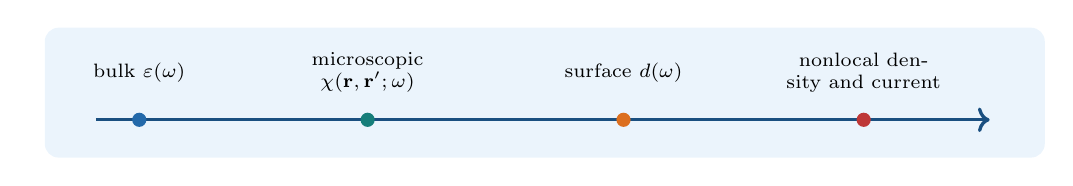
\begin{tikzpicture}[x=1cm,y=1cm]
    \fill[softblue,rounded corners=5pt] (0,0) rectangle (12.7,1.65);
    \draw[blue!75!black,very thick,->] (0.65,0.48)--(12.0,0.48);
    \foreach \x/\lab/\col in {
      1.2/{bulk $\varepsilon(\omega)$}/blue,
      4.1/{microscopic $\chi(\mathbf r,\mathbf r';\omega)$}/teal,
      7.35/{surface $d(\omega)$}/orange,
      10.4/{nonlocal density and current}/red}{
      \fill[\col] (\x,0.48) circle (0.09);
      \node[font=\scriptsize,align=center,text width=2.6cm] at (\x,1.08){\lab};
    }
  \end{tikzpicture}
  \vfill
  {\large\color{ink}Fedor Shukin\par}
  {\normalsize\color{blue}Journal club \hspace{0.6em}$\cdot$\hspace{0.6em} July 27th 2026\par}
\end{frame}

\begin{frame}{At a nanometre, the boundary is no longer a line}
\small
\begin{columns}[T,onlytextwidth]
  \column{0.58\textwidth}
  \centering
  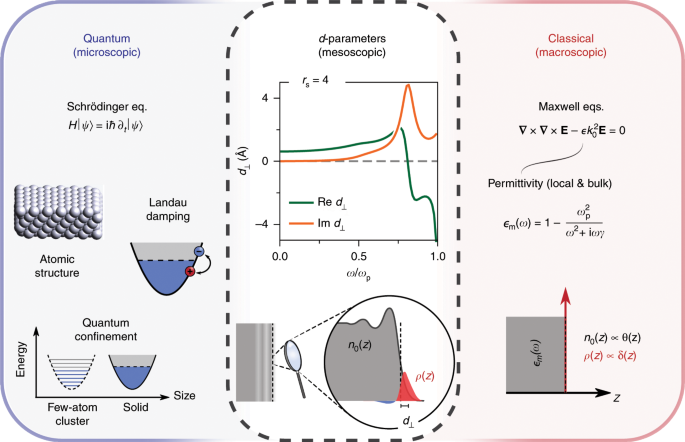
\includegraphics[
    width=\linewidth,
    height=0.60\textheight,
    keepaspectratio
  ]{assets/goncalves2020_fig1.png}
  \shortcite{P. A. D. Gonçalves et al., Nat. Commun. 11, 366 (2020), Fig. 1.}
  \column{0.37\textwidth}
  \begin{block}{The central question}
    How do we keep the useful scale of Maxwell solvers when the electronic structure of the boundary becomes observable?
  \end{block}
  \begin{itemize}
    \item Local optics places induced charge on an ideal surface.
    \item Nanometre confinement resolves the charge centroid, spill-out, and longitudinal motion.
    \item Tunnelling can remove the dielectric boundary altogether.
  \end{itemize}
  \vspace{0.2em}
  {\normalsize\color{teal!80!black}\bfseries The interface becomes part of the material model.}
\end{columns}
\end{frame}

\begin{frame}{The route from Maxwell to a mesoscopic model}
\centering
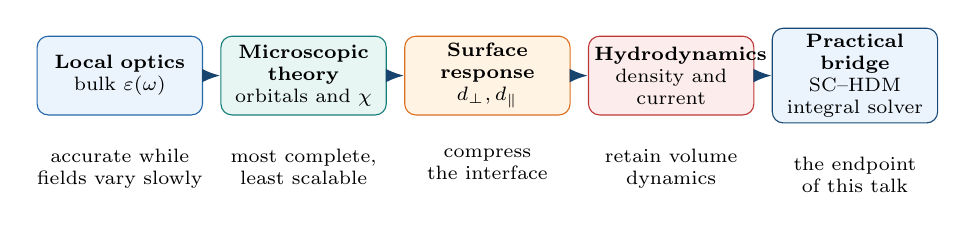
\begin{tikzpicture}[node distance=0.22cm, every node/.style={align=center,font=\scriptsize,text width=1.95cm,inner sep=2pt}]
  \node[draw=blue,fill=softblue,rounded corners,minimum width=2.1cm,minimum height=1.0cm] (a)
    {\textbf{Local optics}\\bulk $\varepsilon(\omega)$};
  \node[draw=teal,fill=softteal,rounded corners,minimum width=2.1cm,minimum height=1.0cm,right=of a] (b)
    {\textbf{Microscopic theory}\\orbitals and $\chi$};
  \node[draw=orange,fill=softorange,rounded corners,minimum width=2.1cm,minimum height=1.0cm,right=of b] (c)
    {\textbf{Surface response}\\$d_\perp,d_\parallel$};
  \node[draw=red,fill=softred,rounded corners,minimum width=2.1cm,minimum height=1.0cm,right=of c] (d)
    {\textbf{Hydrodynamics}\\density and current};
  \node[draw=blue!70!black,fill=softblue,rounded corners,minimum width=2.1cm,minimum height=1.0cm,right=of d] (e)
    {\textbf{Practical bridge}\\SC--HDM integral solver};
  \foreach \x/\y in {a/b,b/c,c/d,d/e}{\draw[-{Latex},thick,blue!65!black] (\x)--(\y);}
  \node[below=0.35cm of a,font=\scriptsize,text width=2.2cm]{accurate while fields vary slowly};
  \node[below=0.35cm of b,font=\scriptsize,text width=2.2cm]{most complete, least scalable};
  \node[below=0.35cm of c,font=\scriptsize,text width=2.2cm]{compress the interface};
  \node[below=0.35cm of d,font=\scriptsize,text width=2.2cm]{retain volume dynamics};
  \node[below=0.35cm of e,font=\scriptsize,text width=2.2cm]{the endpoint of this talk};
\end{tikzpicture}
\vspace{0.8em}
\begin{block}{The storyline}
  Each step keeps more electronic structure than the previous one, but the useful model is the least expensive response object that still contains the missing physics.
\end{block}
\end{frame}

\begin{frame}{Classical local optics: the successful baseline}
\footnotesize
\begin{columns}[T,onlytextwidth]
  \column{0.49\textwidth}
  \begin{block}{Local constitutive law}
    \[
      \mathbf P=\varepsilon_0\chi(\omega)\mathbf E,\qquad
      \mathbf J=\sigma(\omega)\mathbf E,
    \]
    \[
      \varepsilon_m=\varepsilon_\infty-\frac{\omega_p^2}{\omega(\omega+i\gamma)}.
    \]
  \end{block}
  \begin{block}{The controlled scale separation}
    $\omega\tau_e\ll1$ and $\ell_e/L_{\rm field}\ll1$, with
    $\tau_e\sim\omega_p^{-1}$ or $\hbar/E_F$ and $\ell_e$ a screening / spill-out scale.
  \end{block}
  \begin{itemize}
    \item Geometry, radiation, retardation, and bulk absorption can all be treated accurately.
    \item The induced charge is assigned to a mathematically sharp interface; refining the mesh does not change that constitutive assumption.
  \end{itemize}
  \column{0.46\textwidth}
  \centering
  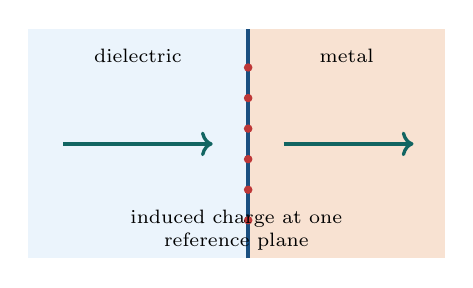
\begin{tikzpicture}[x=1cm,y=0.97cm]
    \fill[softblue] (0,0) rectangle (5.3,3.0);
    \fill[orange!20] (2.8,0) rectangle (5.3,3.0);
    \draw[blue!75!black,very thick] (2.8,0)--(2.8,3.0);
    \foreach \y in {0.5,0.9,...,2.55}{\fill[red] (2.8,\y) circle (0.055);}
    \draw[teal!80!black,very thick,->] (0.45,1.5)--(2.35,1.5);
    \draw[teal!80!black,very thick,->] (3.25,1.5)--(4.9,1.5);
    \node[font=\scriptsize] at (1.4,2.65){dielectric};
    \node[font=\scriptsize] at (4.05,2.65){metal};
    \node[font=\scriptsize,align=center,text width=4.3cm] at (2.65,0.37)
      {induced charge at one\\reference plane};
  \end{tikzpicture}
  \begin{alertblock}{The hidden approximation}
    The material remembers frequency, but not wavevector, surface structure, or connectivity.
  \end{alertblock}
\end{columns}
\vspace{-0.15em}
\end{frame}

\begin{frame}{A large antenna can contain an atomic-scale optical gap}
\small
\begin{columns}[T,onlytextwidth]
  \column{0.54\textwidth}
  \centering
  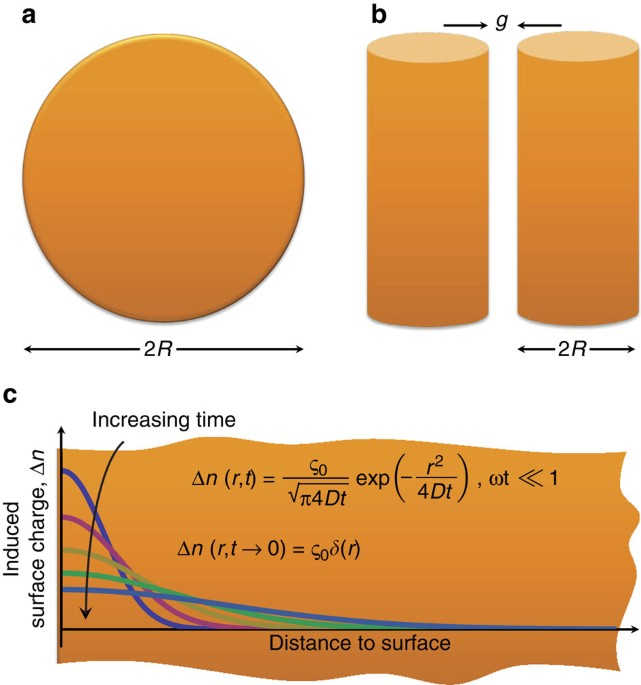
\includegraphics[
    width=0.76\linewidth,
    height=0.52\textheight,
    keepaspectratio,
    trim=305bp 258bp 0bp 0bp,
    clip
  ]{assets/mortensen2014_fig1.jpg}
  \shortcite{N. A. Mortensen et al., Nat. Commun. 5, 3809 (2014), Fig. 1(b).}
  \column{0.42\textwidth}
  \begin{block}{The geometric scales}
    $R$: radius / curvature;\quad $g$: facing-surface dielectric gap;\quad
    $t$: thickness of a film, sheet, or spacer stack.
  \end{block}
  \begin{alertblock}{Why the gap wins}
    A wide antenna can still have $g,t\sim1$ nm, producing $q\sim1/g$ or $q_z\sim1/t$.
  \end{alertblock}
  \key{The relevant size is the shortest dimension sampled by the field, not the overall footprint.}
\end{columns}
\end{frame}

\begin{frame}{Breakdown is controlled by the smallest field scale}
\small
\begin{columns}[T,onlytextwidth]
  \column{0.49\textwidth}
  \begin{block}{The relevant comparisons}
    \[
      q\ell,\qquad \frac{\ell}{R},\qquad \frac{\ell}{g},\qquad \frac{\ell}{t}.
    \]
    Here $\ell$ can be a screening length, spill-out width, Fermi wavelength, mean free path, tunnelling length, or exciton radius.
  \end{block}
  \begin{itemize}
    \item A $100$-nm antenna with a $1$-nm gap contains $q\sim 1/g$ field components.
    \item A large particle can therefore be more nonlocal than a smaller, weakly confined one.
    \item Resonance shifts alone are ambiguous: geometry, chemistry, nonlocality, and spill-out can imitate one another.
  \end{itemize}
  \column{0.47\textwidth}
  \centering
  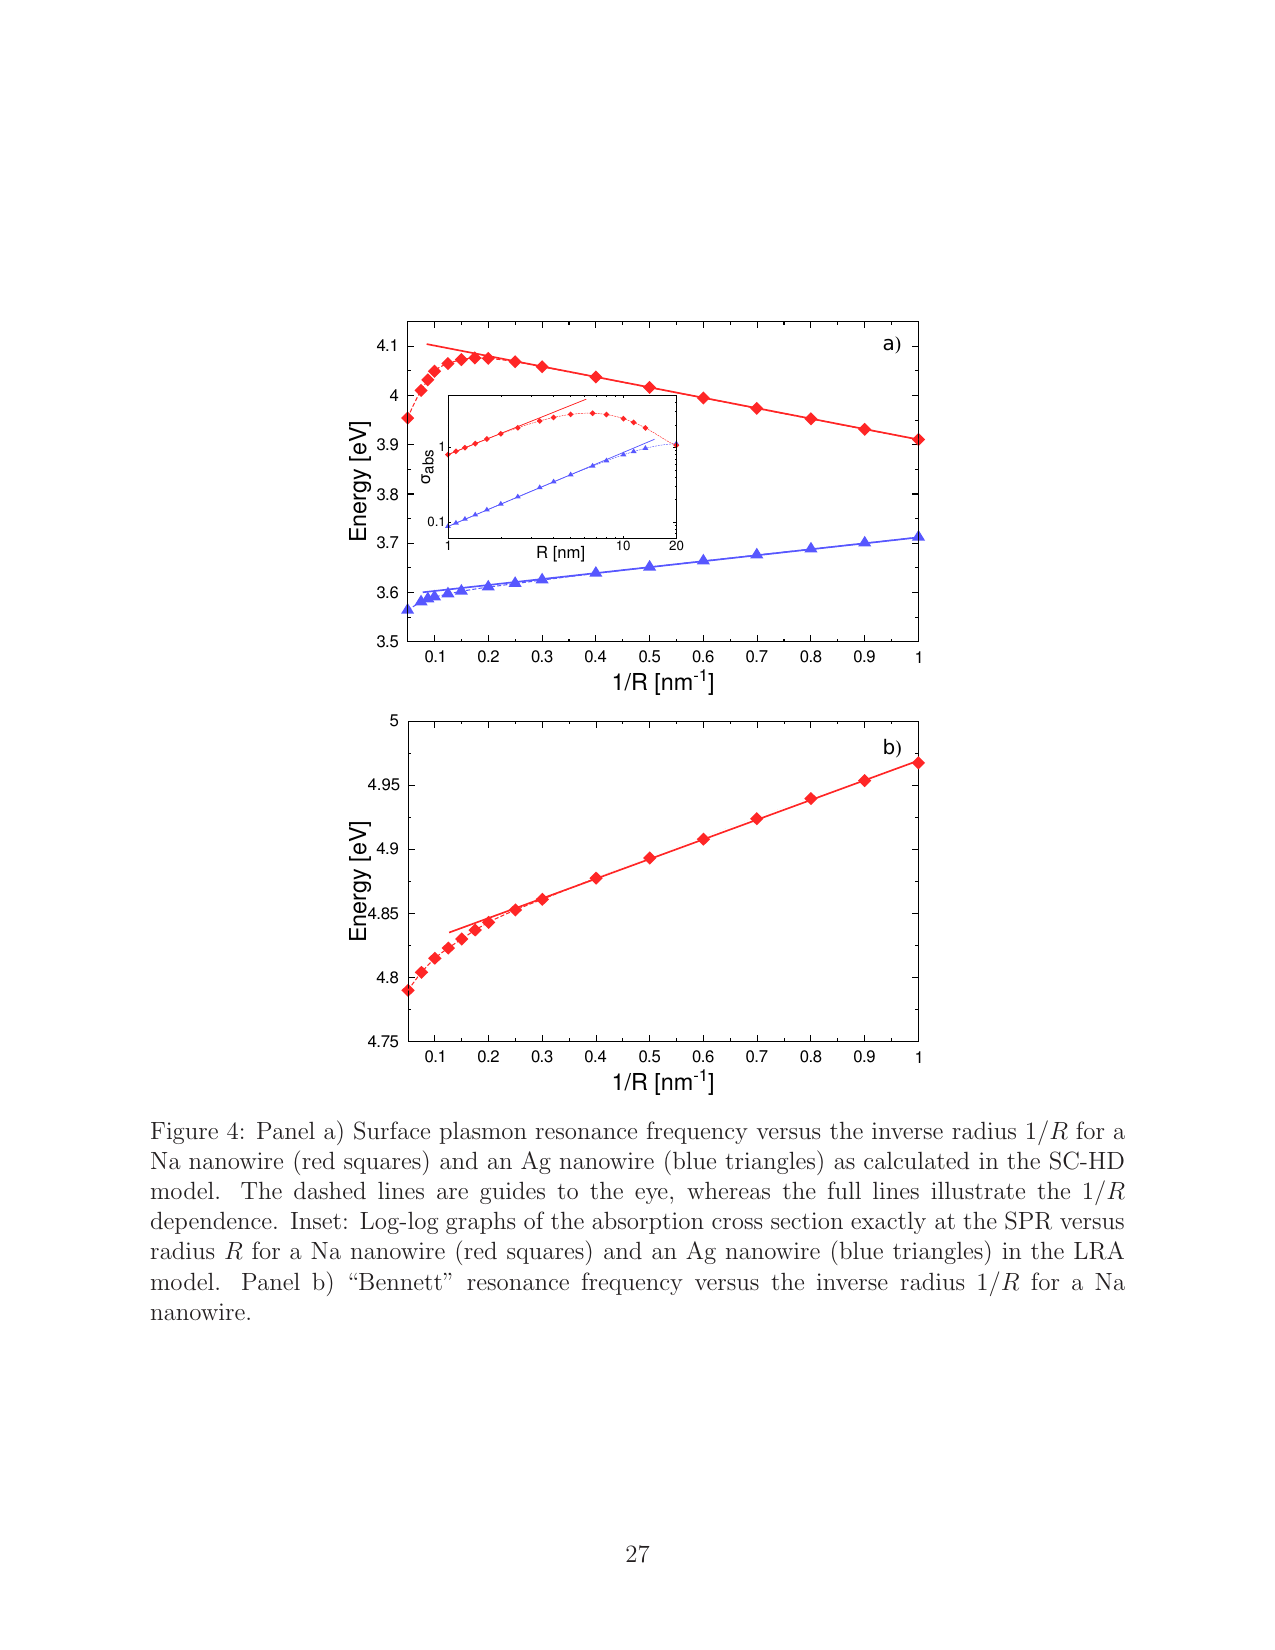
\includegraphics[
    width=\linewidth,
    height=0.60\textheight,
    keepaspectratio,
    trim=151bp 259bp 161bp 145bp,
    clip
  ]{assets/toscano2015_fig4_page.png}
  \shortcite{G. Toscano et al., Nat. Commun. 6, 7132 (2015), Fig. 4.}
\end{columns}
\end{frame}

\begin{frame}{Nanoparticles and 2D materials expose different nonlocalities}
\scriptsize
\begin{columns}[T,onlytextwidth]
  \column{0.48\textwidth}
  \begin{block}{Finite metal nanoparticles}
    \begin{itemize}
      \item Surface-to-volume ratio grows as size decreases.
      \item Discrete electron--hole transitions coexist with collective plasmons.
      \item Facets, $d$-band screening, spill-out, and curvature affect the same spectrum.
    \end{itemize}
  \end{block}
  \centering
  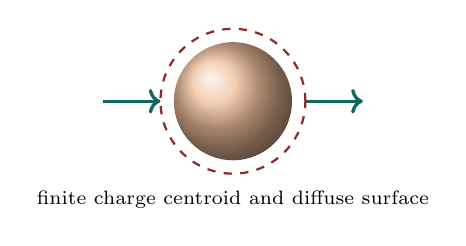
\begin{tikzpicture}
    \shade[ball color=orange!45] (0,0) circle (0.75);
    \draw[teal!80!black,very thick,->] (-1.65,0)--(-0.92,0);
    \draw[teal!80!black,very thick,->] (0.92,0)--(1.65,0);
    \draw[red!75!black,dashed,thick] (0,0) circle (0.92);
    \node[font=\scriptsize] at (0,-1.25){finite charge centroid and diffuse surface};
  \end{tikzpicture}
  \column{0.48\textwidth}
  \begin{alertblock}{Atomically thin conductors and excitons}
    \begin{itemize}
      \item The response is naturally $\sigma_{2D}(q,\omega)$ or $\chi_{2D}(q,\omega)$.
      \item Large-$q$ plasmons sample the Fermi surface and Landau-damping continuum.
      \item Exciton dispersion and finite coherence length make a local sheet susceptibility incomplete.
      \item Finite out-of-plane polarizability, $J_z(z)$, and spill-out shift the transverse screening centroid, especially near substrates or in TM near fields.
    \end{itemize}
  \end{alertblock}
  \centering
  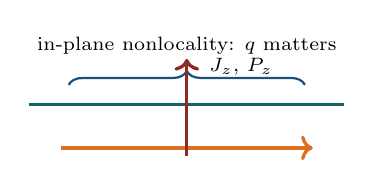
\begin{tikzpicture}
    \draw[teal!80!black,very thick] (-2,0)--(2,0);
    \draw[blue!75!black,thick,decorate,decoration={brace,amplitude=5pt}] (-1.5,0.25)--(1.5,0.25);
    \node[font=\scriptsize] at (0,0.75){in-plane nonlocality: $q$ matters};
    \draw[orange,very thick,->] (-1.6,-0.55)--(1.6,-0.55);
    \draw[red!75!black,very thick,->] (0,-0.65)--(0,0.58);
    \node[font=\scriptsize,anchor=west] at (0.16,0.48){$J_z,\,P_z$};
  \end{tikzpicture}
\end{columns}
\shortcite{M. Jablan et al., Phys. Rev. B 80, 245435 (2009); M. B. Lundeberg et al., Science 357, 187 (2017); H. C. Nerl et al., Nat. Commun. 15, 1 (2024).}
\end{frame}

\begin{frame}{The microscopic route: orbitals, screening, and correlations}
\small
\begin{columns}[T,onlytextwidth]
  \column{0.61\textwidth}
  \centering
  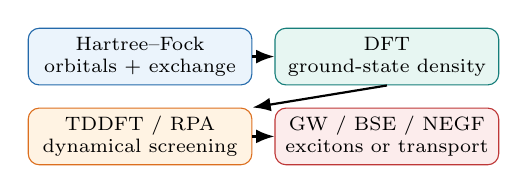
\begin{tikzpicture}[node distance=0.28cm,every node/.style={font=\scriptsize,align=center,text width=2.7cm,minimum height=0.72cm,inner sep=2pt}]
    \node[draw=blue,fill=softblue,rounded corners] (hf){Hartree--Fock\\orbitals + exchange};
    \node[draw=teal,fill=softteal,rounded corners,right=of hf] (dft){DFT\\ground-state density};
    \node[draw=orange,fill=softorange,rounded corners,below=of hf] (tddft){TDDFT / RPA\\dynamical screening};
    \node[draw=red,fill=softred,rounded corners,right=of tddft] (mb){GW / BSE / NEGF\\excitons or transport};
    \draw[-{Latex},thick] (hf)--(dft);
    \draw[-{Latex},thick] (dft.south)--(tddft.north east);
    \draw[-{Latex},thick] (tddft)--(mb);
  \end{tikzpicture}
  \vspace{0.65em}
  \begin{block}{The microscopic response object}
    \[
      \delta n(\mathbf r,\omega)
      =\int \chi(\mathbf r,\mathbf r';\omega)\,
      \delta v_{\rm ext}(\mathbf r',\omega)\,d\mathbf r'.
    \]
    Atomic geometry, discrete transitions, surface states, spill-out, and tunnelling can all enter $\chi$.
  \end{block}
  \column{0.35\textwidth}
  \begin{itemize}
    \item HF and DFT provide orbitals or densities, but are not exact many-body theories.
    \item TDDFT and RPA add dynamical screening.
    \item GW/BSE improves quasiparticles and excitons.
    \item NEGF treats open boundaries and transport.
  \end{itemize}
  \begin{alertblock}{Why use them here?}
    They are the reference for deciding which electronic information a cheaper model must retain.
  \end{alertblock}
\end{columns}
\shortcite{E. Runge and E. K. U. Gross, Phys. Rev. Lett. 52, 997 (1984); G. Onida et al., Rev. Mod. Phys. 74, 601 (2002).}
\end{frame}

\begin{frame}{Atoms reorganize the optical spectrum}
\footnotesize
\begin{columns}[T,onlytextwidth]
  \column{0.59\textwidth}
  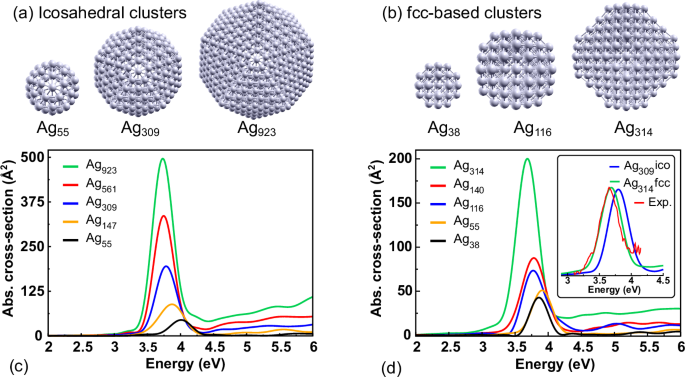
\includegraphics[width=\linewidth,height=0.64\textheight,keepaspectratio]{assets/chaudhary2024_fig2.png}
  \shortcite{M. Chaudhary and H.-C. Weissker, Nat. Commun. 15, 9225 (2024), Fig. 2.}
  \column{0.37\textwidth}
  \begin{block}{What the calculation shows}
    RT--TDDFT+$U$ retains atomic geometry and filled-$d$ screening while following Ag clusters toward a collective response.
  \end{block}
  \begin{itemize}
    \item Small clusters have discrete electron--hole peaks.
    \item Larger clusters develop a broad LSPR.
    \item Icosahedral and fcc-based particles do not produce identical spectra.
    \item One electronic model is used across the size sequence.
  \end{itemize}
  \begin{alertblock}{The remaining difficulty}
    Even this unusually large calculation reaches only a few nanometres—far below a realistic device sweep.
  \end{alertblock}
\end{columns}
\end{frame}

\begin{frame}{A collective plasmon emerges—but not as a universal curve}
\footnotesize
\begin{columns}[T,onlytextwidth]
  \column{0.61\textwidth}
  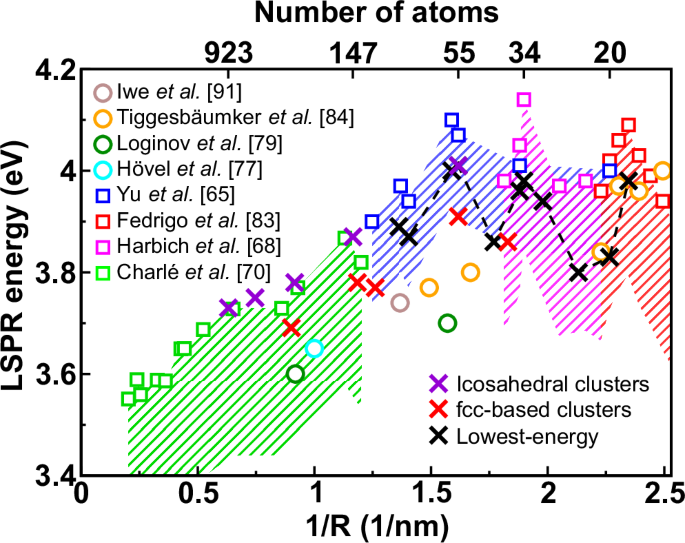
\includegraphics[width=\linewidth,height=0.65\textheight,keepaspectratio]{assets/chaudhary2024_fig3.png}
  \shortcite{M. Chaudhary and H.-C. Weissker, Nat. Commun. 15, 9225 (2024), Fig. 3.}
  \column{0.35\textwidth}
  \begin{block}{Size trend}
    The LSPR energy varies systematically with inverse radius from Ag$_4$ to Ag$_{923}$.
  \end{block}
  \begin{itemize}
    \item The smallest systems retain discrete structure.
    \item The large-cluster limit becomes collective.
    \item Shape families remain separated at comparable size.
    \item A fitted size correction would mix confinement, geometry, and $d$-band screening.
  \end{itemize}
  \vspace{0.2em}
  \key{The microscopic result is a benchmark, not yet a transferable constitutive law.}
\end{columns}
\end{frame}

\begin{frame}{Microscopic quantum models do not scale}
\begin{columns}[T,onlytextwidth]
  \column{0.47\textwidth}
  \begin{block}{What becomes expensive}
    \begin{itemize}
      \item thousands of atoms and thousands of active electrons;
      \item many frequencies, shapes, gaps, substrates, and disorder realizations;
      \item long-range electromagnetic domains around a microscopic region;
      \item open-system transport or many-body linewidths.
    \end{itemize}
  \end{block}
  \column{0.49\textwidth}
  \begin{alertblock}{The transfer problem}
    A microscopic spectrum answers one geometry. A device model needs a compact response object that can be reused in BEM, FEM, or an integral solver.
  \end{alertblock}
  \vspace{0.35em}
  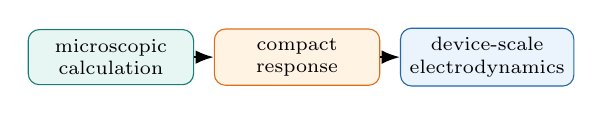
\begin{tikzpicture}[node distance=0.25cm,every node/.style={font=\scriptsize,align=center}]
    \node[draw=teal,fill=softteal,rounded corners,minimum width=2.1cm,minimum height=0.7cm] (a){microscopic\\calculation};
    \node[draw=orange,fill=softorange,rounded corners,minimum width=2.1cm,minimum height=0.7cm,right=of a] (b){compact\\response};
    \node[draw=blue,fill=softblue,rounded corners,minimum width=2.1cm,minimum height=0.7cm,right=of b] (c){device-scale\\electrodynamics};
    \draw[-{Latex},thick] (a)--(b);
    \draw[-{Latex},thick] (b)--(c);
  \end{tikzpicture}
  \vspace{0.4em}
  \key{Mesoscopic modelling begins at this compression step.}
\end{columns}
\shortcite{M. Chaudhary and H.-C. Weissker, Nat. Commun. 15, 9225 (2024).}
\end{frame}

\begin{frame}{Before tunnelling, the screening charge has already moved}
\scriptsize
\begin{columns}[T,onlytextwidth]
  \column{0.60\textwidth}
  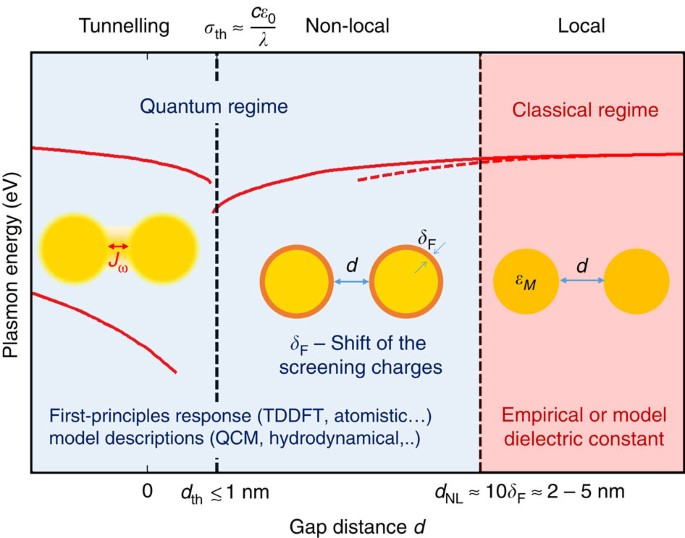
\includegraphics[width=\linewidth,height=0.64\textheight,keepaspectratio]{assets/zhu2016_fig1.jpg}
  \shortcite{W. Zhu et al., Nat. Commun. 7, 11495 (2016), Fig. 1.}
  \column{0.36\textwidth}
  \begin{block}{Three gap regimes}
    \begin{enumerate}
      \item \textbf{Local:} the geometric and optical gaps coincide.
      \item \textbf{Nonlocal:} at $d\lesssim d_{\rm NL}\sim10\delta_F\approx2$--$5$ nm, the screening centroid shifts by the Fermi-scale distance $\delta_F$, changing the optical gap.
      \item \textbf{Tunnelling:} below the threshold $d_{\rm th}\lesssim1$ nm, an ac conductance $\sigma_{\rm th}\simeq c\varepsilon_0/\lambda$ crosses the gap and charge-transfer modes appear.
    \end{enumerate}
  \end{block}
  \begin{alertblock}{The key distinction}
    Surface response can correct two separated bodies. Once the junction conducts, the boundary conditions themselves change.
  \end{alertblock}
\end{columns}
\end{frame}

\begin{frame}{Compressing a quantum interface into two response functions}
\small
\begin{columns}[T,onlytextwidth]
  \column{0.48\textwidth}
  \begin{block}{Perpendicular charge centroid}
    \[
      d_\perp(\omega)=
      \frac{\int z\,\rho_{\rm ind}(z,\omega)\,dz}
           {\int \rho_{\rm ind}(z,\omega)\,dz}.
    \]
    \[
      d_\parallel(\omega)=
      \frac{\int z\,\partial_zJ_x(z,\omega)\,dz}
           {\int \partial_zJ_x(z,\omega)\,dz},
      \quad J_x\parallel\text{ interface}.
    \]
  \end{block}
  \begin{itemize}
    \item $\operatorname{Re}d$ changes phase and resonance energy.
    \item $\operatorname{Im}d$ contributes surface-enabled loss.
    \item The reference plane and sign convention must be specified.
  \end{itemize}
  \column{0.48\textwidth}
  \centering
  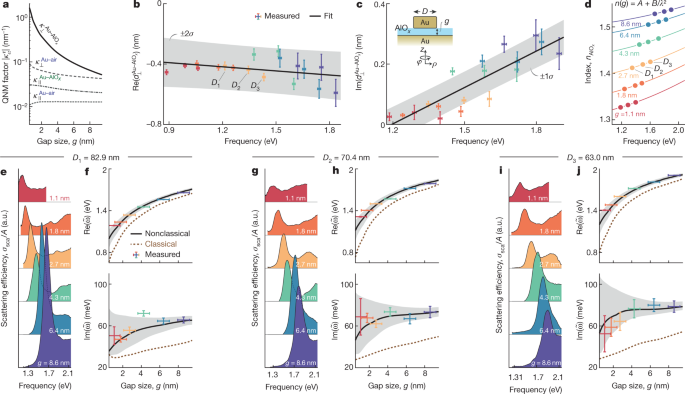
\includegraphics[
    width=\linewidth,
    height=0.38\textheight,
    keepaspectratio,
    trim=160bp 244bp 110bp 0bp,
    clip
  ]{assets/yang2019_fig3_lw685.png}
  \shortcite{Y. Yang et al., Nature 576, 248 (2019), Fig. 3(b,c).}
  \begin{alertblock}{What has been gained}
    An atomically structured interface becomes a boundary correction that can be inserted into a classical solver.
  \end{alertblock}
\end{columns}
\end{frame}

\begin{frame}{The surface response is complex, dispersive, and measurable}
\footnotesize
\begin{columns}[T,onlytextwidth]
  \column{0.62\textwidth}
  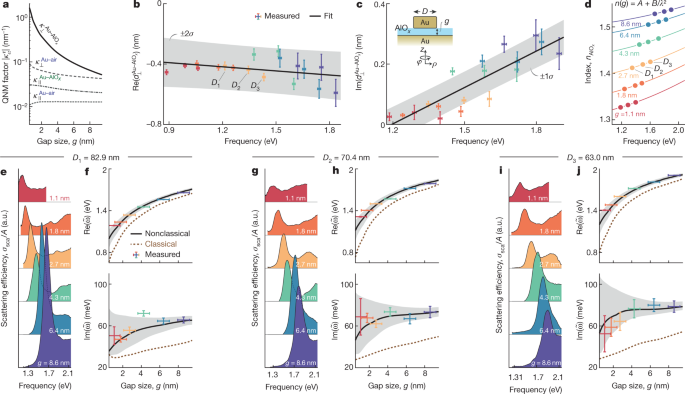
\includegraphics[width=\linewidth,height=0.63\textheight,keepaspectratio]{assets/yang2019_fig3_lw685.png}
  \shortcite{Y. Yang et al., Nature 576, 248 (2019), Fig. 3.}
  \column{0.34\textwidth}
  \begin{block}{Experimental retrieval}
    Families of film-coupled resonators provide resonance shifts and linewidths from which a complex Au--AlO$_x$ $d_\perp(\omega)$ is inferred.
  \end{block}
  \begin{itemize}
    \item The response varies with frequency; it is not one fitted length.
    \item Nonclassical shifts exceed 30\% in the reported architecture.
    \item Using both shift and linewidth tests reactive and dissipative response.
    \item Transfer still depends on facet, reference plane, and wavevector.
  \end{itemize}
\end{columns}
\end{frame}

\begin{frame}{Spill-out starts in the ground state}
\small
\begin{columns}[T,onlytextwidth]
  \column{0.53\textwidth}
  \centering
  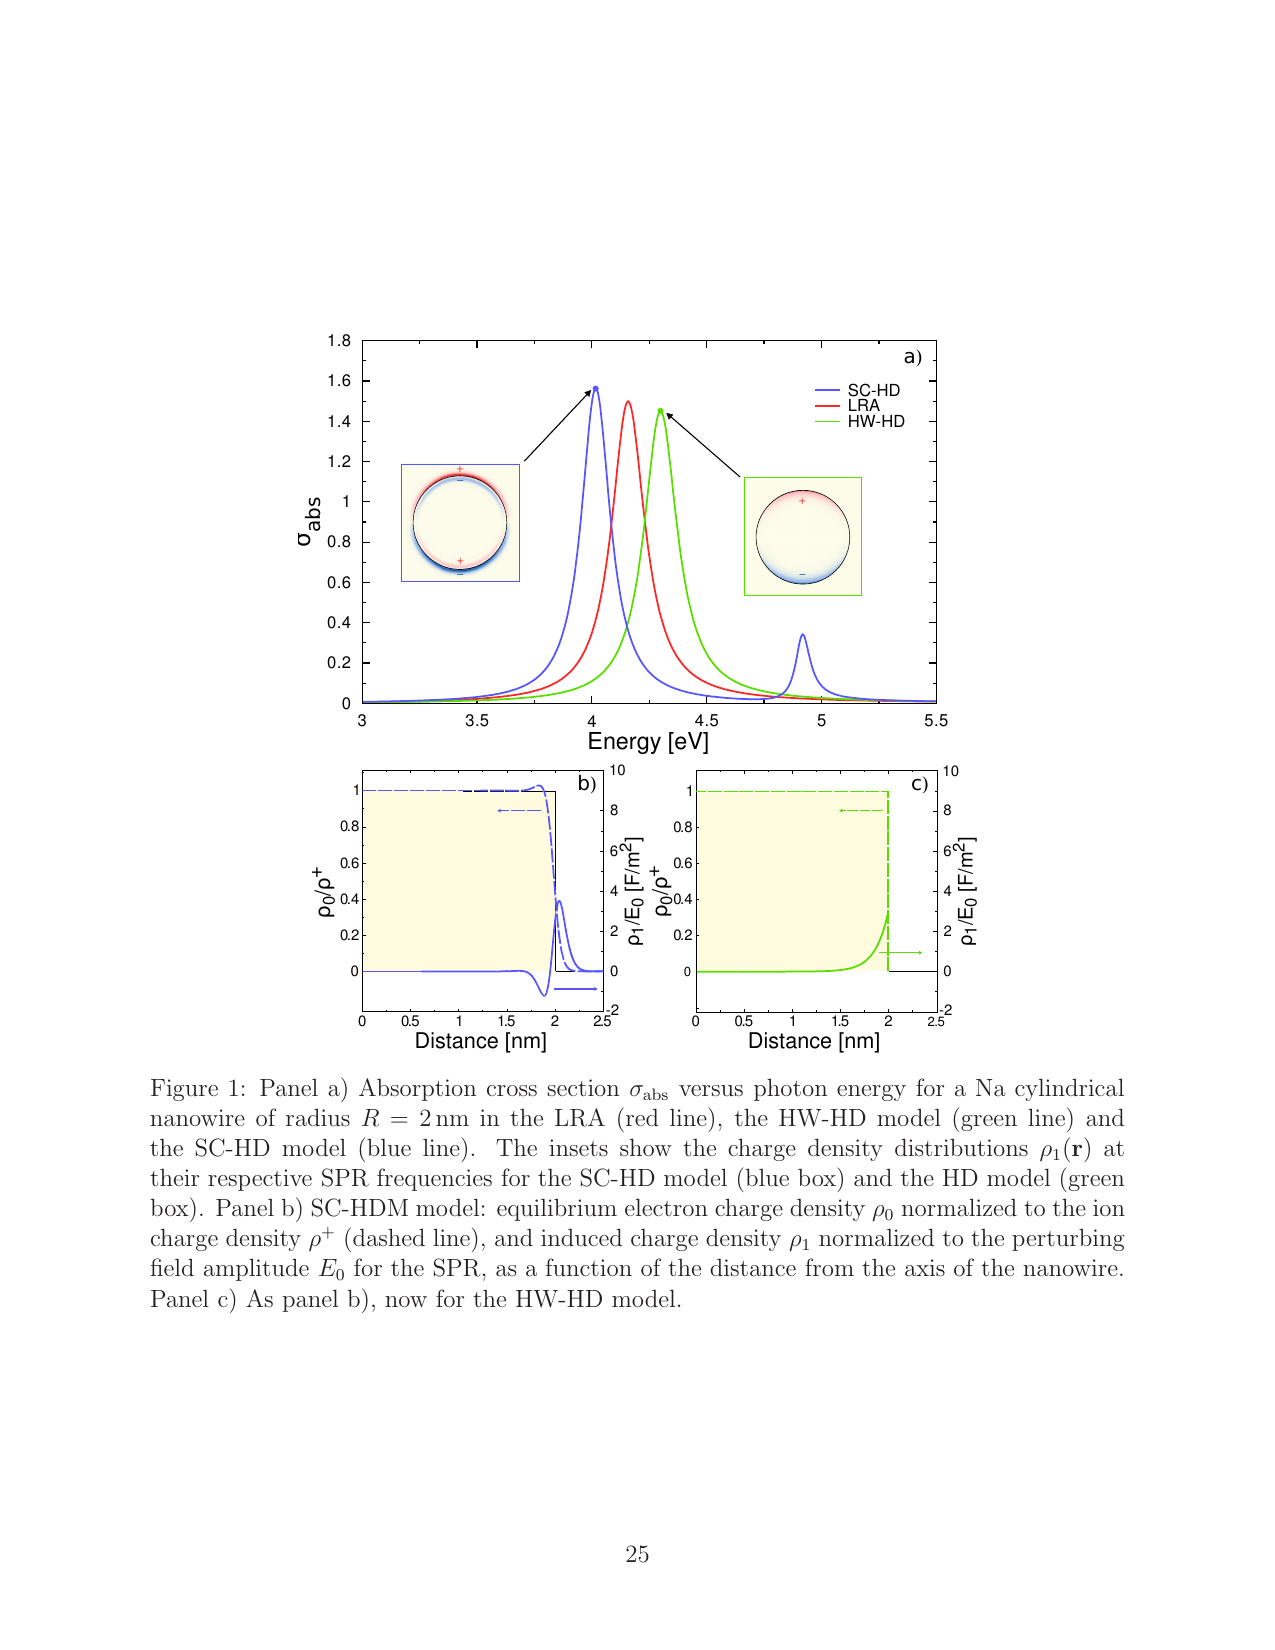
\includegraphics[
    width=\linewidth,
    height=0.42\textheight,
    keepaspectratio,
    trim=145bp 286bp 147bp 366bp,
    clip
  ]{assets/toscano2015_fig1_page.png}
  \shortcite{G. Toscano et al., Nat. Commun. 6, 7132 (2015), Fig. 1(b,c).}
  \column{0.43\textwidth}
  \begin{block}{Equilibrium inhomogeneity}
    A smooth $n_0(z)$ creates a finite-width induced charge and a nonzero surface centroid even if the constitutive response is local pointwise.
  \end{block}
  \begin{itemize}
    \item Spill-out or spill-in is a ground-state property.
    \item Electron-gas compressibility is a dynamical nonlocal property.
    \item Their spectral shifts can reinforce or cancel.
    \item Facets, Friedel oscillations, and correlations remain material dependent.
  \end{itemize}
\end{columns}
\end{frame}

\begin{frame}{Compute the interface once; reuse it in Maxwell solvers}
\small
\centering
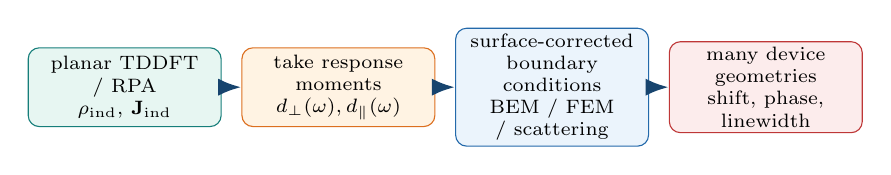
\begin{tikzpicture}[node distance=0.25cm,every node/.style={font=\scriptsize,align=center,text width=2.25cm,inner sep=2pt}]
  \node[draw=teal,fill=softteal,rounded corners,minimum width=2.45cm,minimum height=1.0cm] (a)
    {planar TDDFT / RPA\\$\rho_{\rm ind},\,\mathbf J_{\rm ind}$};
  \node[draw=orange,fill=softorange,rounded corners,minimum width=2.45cm,minimum height=1.0cm,right=of a] (b)
    {take response moments\\$d_\perp(\omega),d_\parallel(\omega)$};
  \node[draw=blue,fill=softblue,rounded corners,minimum width=2.45cm,minimum height=1.0cm,right=of b] (c)
    {surface-corrected\\boundary conditions\\BEM / FEM / scattering};
  \node[draw=red,fill=softred,rounded corners,minimum width=2.45cm,minimum height=1.0cm,right=of c] (d)
    {many device geometries\\shift, phase, linewidth};
  \foreach \x/\y in {a/b,b/c,c/d}{\draw[-{Latex},very thick,blue!65!black] (\x)--(\y);}
\end{tikzpicture}
\vspace{0.55em}
\begin{columns}[T,onlytextwidth]
  \column{0.50\textwidth}
  \begin{block}{Why this is mesoscopic}
    The atomic-scale calculation is retained through a small number of frequency-dependent surface functions rather than through every orbital.
  \end{block}
  \begin{block}{Leading modified boundary conditions}
    \scriptsize With $[\![f]\!]=f_{\rm d}-f_{\rm m}$,
    \[
      [\![\mathbf E_\parallel]\!]=-d_\perp\nabla_\parallel[\![E_\perp]\!],
      \qquad
      [\![D_\perp]\!]=d_\parallel\nabla_\parallel\!\cdot\![\![\mathbf D_\parallel]\!] .
    \]
  \end{block}
  \column{0.46\textwidth}
  \begin{alertblock}{Where the compression can fail}
    Strong curvature, finite $q$ dependence, multiple facets, chemistry, or charge transfer can make a planar first-order $d$ insufficient.
  \end{alertblock}
\end{columns}
\shortcite{P. J. Feibelman, Prog. Surf. Sci. 12, 287 (1982); Y. Yang et al., Nature 576, 248 (2019).}
\end{frame}

\begin{frame}{Tunnelling changes the topology of the boundary}
\small
\begin{columns}[T,onlytextwidth]
  \column{0.60\textwidth}
  \centering
  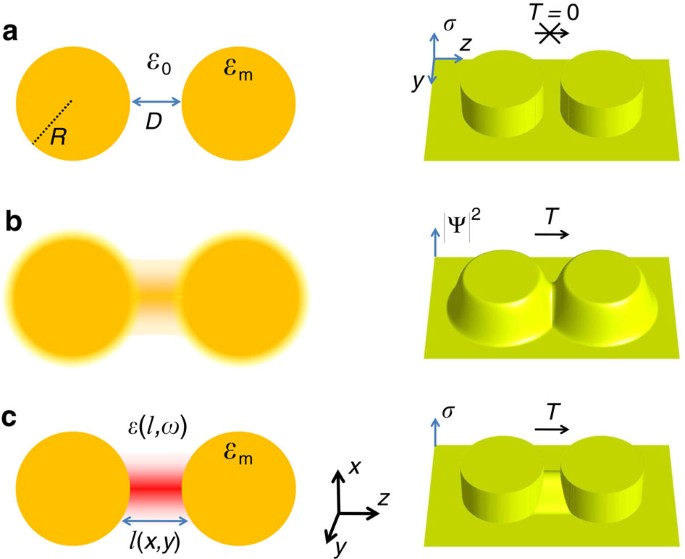
\includegraphics[
    width=\linewidth,
    height=0.69\textheight,
    keepaspectratio
  ]{assets/esteban2012_fig1.jpg}
  \shortcite{R. Esteban et al., Nat. Commun. 3, 825 (2012), Fig. 1.}
  \column{0.36\textwidth}
  \begin{block}{Three descriptions of one junction}
    \begin{itemize}
      \item \textbf{Classical:} $\sigma=0$ in the gap and the tunnelling probability is $T=0$.
      \item \textbf{Quantum:} electronic tails overlap, so $|\Psi|^2$ and $T$ become finite.
      \item \textbf{QCM:} replace the gap by a transport-calibrated $\varepsilon(l,\omega)$.
    \end{itemize}
  \end{block}
  \caution{Model boundary.} Surface response and hard-wall HDM assume separated bodies. A conducting gap instead requires QCM, NEGF, or a transport-calibrated model.
\end{columns}
\end{frame}

\begin{frame}{A surface correction is not yet a bulk nonlocal model}
\footnotesize
\begin{columns}[T,onlytextwidth]
  \column{0.47\textwidth}
  \begin{block}{Surface-response route}
    \[
      \{\rho_{\rm ind}(z),\mathbf J_{\rm ind}(z)\}
      \longrightarrow \{d_\perp,d_\parallel\}.
    \]
    Efficient when the microscopic physics is confined to a thin interface layer.
  \end{block}
  \begin{itemize}
    \item first-order correction about a reference plane;
    \item naturally carries complex surface loss;
    \item easy to reuse in Maxwell solvers.
  \end{itemize}
  \column{0.49\textwidth}
  \begin{alertblock}{Volume-response route}
    \[
      \mathbf J(\mathbf r,\omega)
      \;\hbox{depends on}\;
      \nabla n(\mathbf r,\omega),\ \nabla\!\cdot\!\mathbf J.
    \]
    Needed when $L_{\rm in}\sim\ell_{\rm scr}$: the interior field changes over a screening length and excites longitudinal density motion.
  \end{alertblock}
  \begin{itemize}
    \item retains longitudinal modes and wavevector dependence;
    \item needed for few-nm radii or films, high-order / high-$q$ modes, and extreme gap fields penetrating the metal;
    \item requires an electronic closure and boundary treatment;
    \item leads naturally to quantum hydrodynamics.
  \end{itemize}
\end{columns}
\vspace{0.1em}
\key{Complementary compressions of the same microscopic response.}
\end{frame}

\begin{frame}{Quantum hydrodynamics keeps density and current}
\small
\begin{columns}[T,onlytextwidth]
  \column{0.52\textwidth}
  \begin{block}{Linearized hydrodynamic Drude model}
    \begin{align*}
      -i\omega\,\rho+\nabla\!\cdot\!\mathbf J &=0,\\
      (\gamma-i\omega)\mathbf J &=
      \varepsilon_0\omega_p^2\mathbf E
      -\beta^2\nabla\rho .
    \end{align*}
    The pressure term produces a longitudinal electronic wave and a nonlocal $\varepsilon(\mathbf k,\omega)$.
  \end{block}
  \begin{itemize}
    \item $\beta$ is tied to the Fermi velocity in the simplest closure.
    \item GNOR adds diffusion-like damping.
    \item Maxwell transverse fields couple to longitudinal charge near boundaries.
  \end{itemize}
  \column{0.44\textwidth}
  \centering
  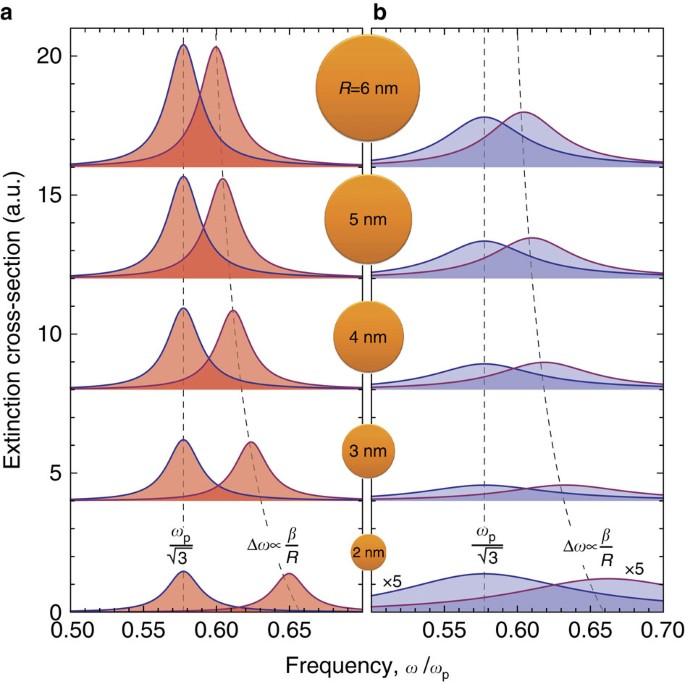
\includegraphics[
    width=\linewidth,
    height=0.70\textheight,
    keepaspectratio
  ]{assets/mortensen2014_fig2.jpg}
  \shortcite{N. A. Mortensen et al., Nat. Commun. 5, 3809 (2014), Fig. 2.}
\end{columns}
\end{frame}

\begin{frame}{Complex gap-mode propagation tests both phase and loss}
\footnotesize
\begin{columns}[T,onlytextwidth]
  \column{0.59\textwidth}
  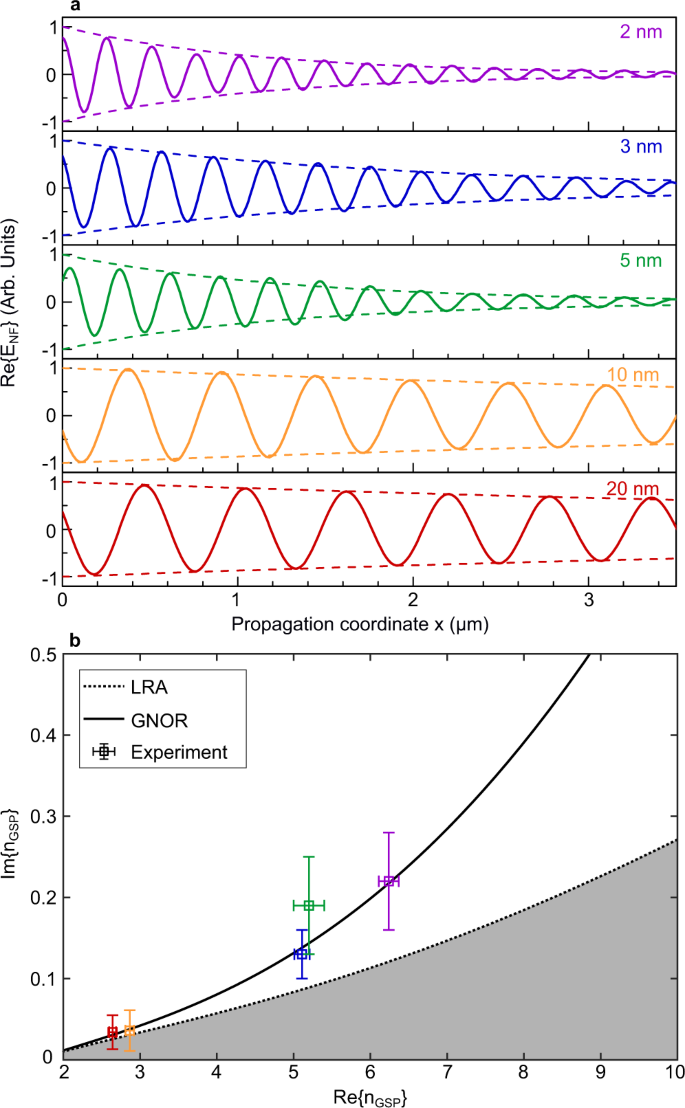
\includegraphics[width=\linewidth,height=0.65\textheight,keepaspectratio]{assets/boroviks2022_fig4.png}
  \shortcite{S. Boroviks et al., Nat. Commun. 13, 3105 (2022), Fig. 4.}
  \column{0.37\textwidth}
  \begin{block}{What is measured}
    s-SNOM retrieves the complex propagation constant of gap plasmons in crystalline Au--Al$_2$O$_3$--Au waveguides.
  \end{block}
  \begin{itemize}
    \item $\operatorname{Re}q$ tracks confinement and phase.
    \item $\operatorname{Im}q$ tracks propagation loss.
    \item Few-nanometre gaps show excess loss relative to LRA.
    \item GNOR reproduces the complex trend with one effective diffusion scale.
  \end{itemize}
  \begin{alertblock}{What the experiment does not fix}
    The fitted diffusion coefficient is an effective closure, not a unique microscopic observable.
  \end{alertblock}
\end{columns}
\end{frame}

\begin{frame}{Hard-wall hydrodynamics moves the problem to the boundary}
\small
\begin{columns}[T,onlytextwidth]
  \column{0.47\textwidth}
  \begin{block}{Standard additional condition}
    \[
      \mathbf J\!\cdot\!\hat{\mathbf n}=0
      \qquad\hbox{at the ionic surface}.
    \]
    The electron fluid is compressed but cannot spill across the chosen boundary.
  \end{block}
  \begin{itemize}
    \item usually produces a blueshift of confined modes;
    \item captures longitudinal pressure waves;
    \item remains inexpensive and stable.
  \end{itemize}
  \column{0.49\textwidth}
  \begin{alertblock}{Physics left outside}
    \begin{itemize}
      \item equilibrium spill-out or spill-in;
      \item facet and atomic chemistry;
      \item interband screening unless added separately;
      \item tunnelling and charge transfer;
      \item a microscopic derivation of phenomenological damping.
    \end{itemize}
  \end{alertblock}
  \vspace{0.2em}
  \caution{A nonlocal equation does not by itself supply a realistic surface.}
\end{columns}
\shortcite{S. Raza et al., J. Phys.: Condens. Matter 27, 183204 (2015).}
\end{frame}

\begin{frame}{Let the equilibrium density define the metal surface}
\small
\begin{columns}[T,onlytextwidth]
  \column{0.51\textwidth}
  \begin{block}{Self-consistent hydrodynamics}
    \begin{enumerate}
      \item Minimize an orbital-free energy functional to obtain $n_0(\mathbf r)$.
      \item Linearize density and current around that diffuse equilibrium.
      \item Couple the induced fields back to Maxwell electrodynamics.
    \end{enumerate}
  \end{block}
  \begin{itemize}
    \item hard-wall HDM: nonlocal dynamics, sharp $n_0$;
    \item SC--HDM / QHT: nonlocal dynamics, diffuse $n_0$;
    \item TDDFT: orbitals and microscopic transitions as well.
  \end{itemize}
  \column{0.45\textwidth}
  \centering
  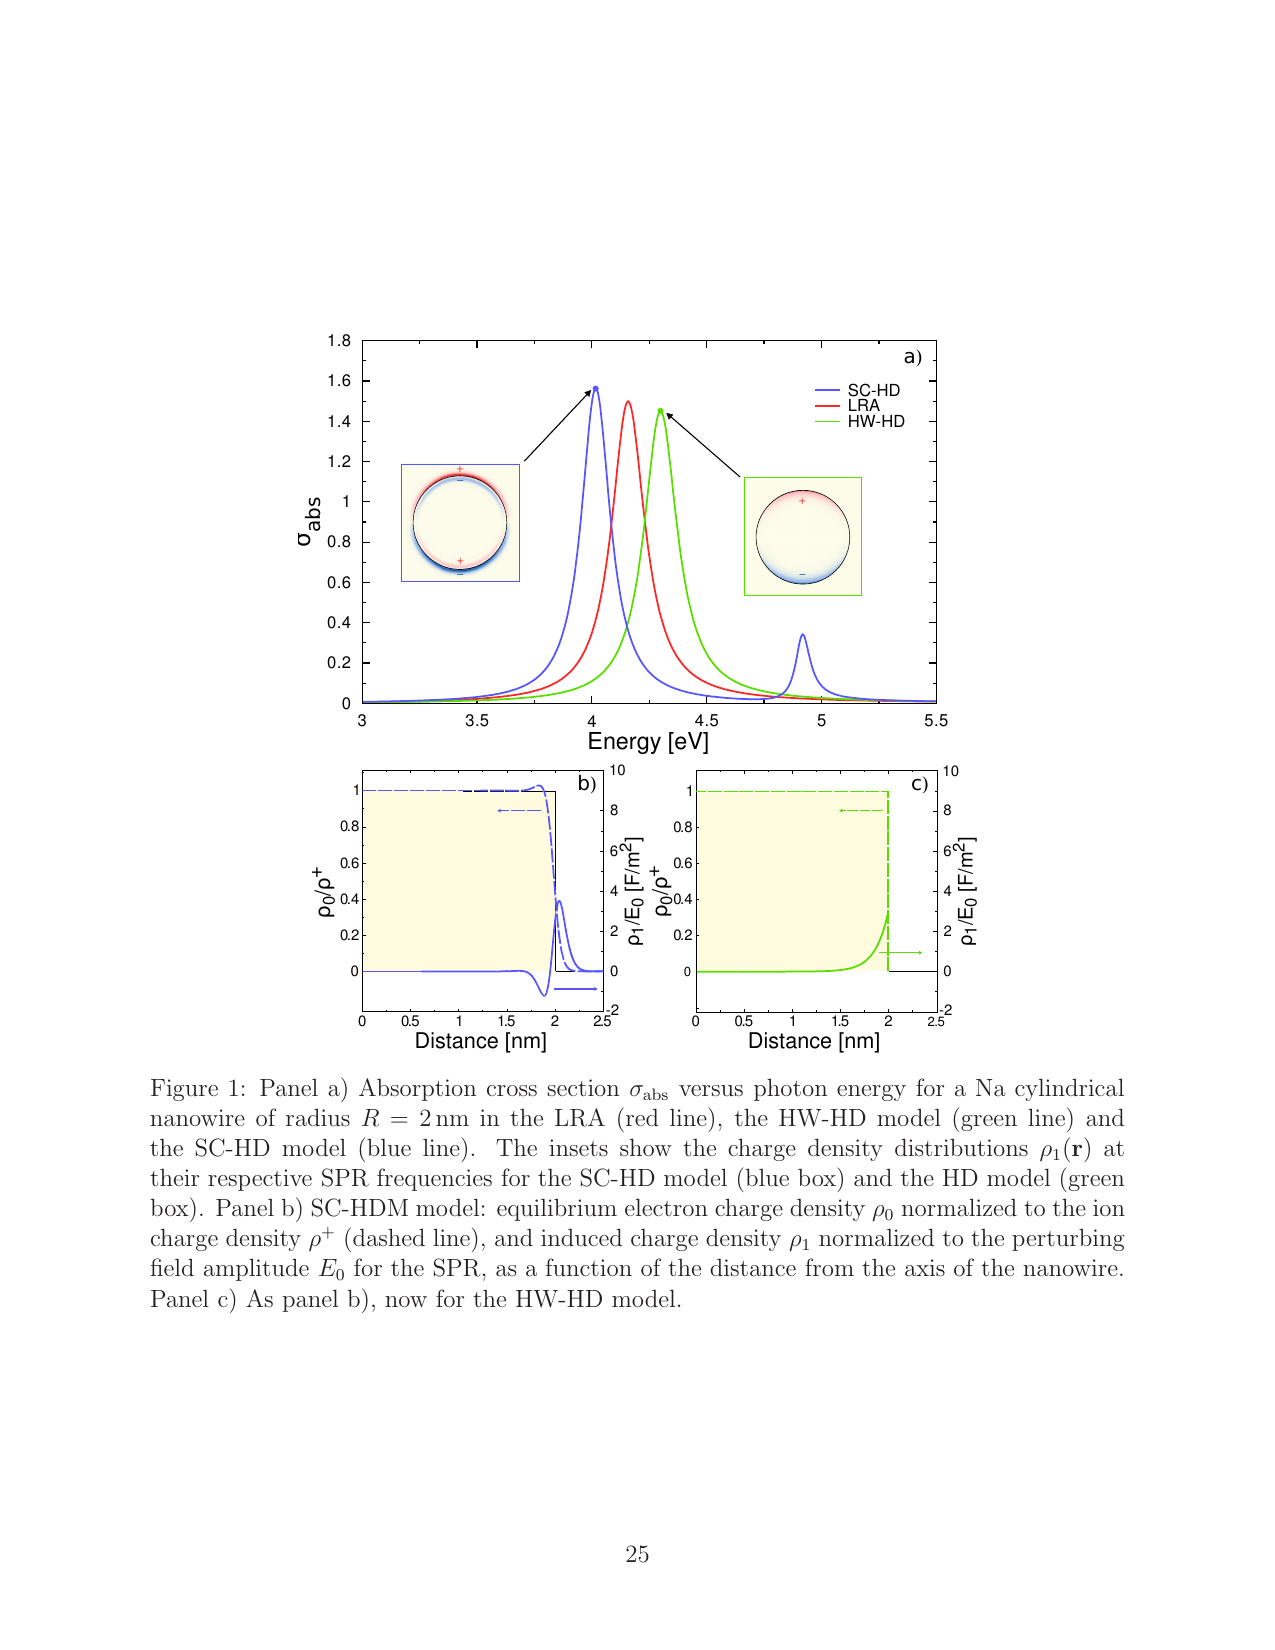
\includegraphics[
    width=\linewidth,
    height=0.39\textheight,
    keepaspectratio,
    trim=145bp 431bp 147bp 159bp,
    clip
  ]{assets/toscano2015_fig1_page.png}
  \shortcite{G. Toscano et al., Nat. Commun. 6, 7132 (2015), Fig. 1(a).}
  \begin{alertblock}{The price}
    Accuracy now depends on the kinetic-energy functional, tail truncation, interband calibration, and numerical treatment of multiple length scales.
  \end{alertblock}
\end{columns}
\end{frame}

\begin{frame}{A spherical volume-integral route removes the exterior mesh}
\small
\begin{columns}[T,onlytextwidth]
  \column{0.39\textwidth}
  \begin{block}{The computational idea}
    \begin{itemize}
      \item Use the homogeneous dyadic Green tensor for radiation.
      \item Expand polarization in vector spherical harmonics.
      \item Represent the diffuse radial density with cubic Lagrange functions.
      \item Separate TE, TM, and longitudinal sectors into radial blocks.
    \end{itemize}
  \end{block}
  \begin{alertblock}{Why the speedup is possible}
    Spherical symmetry reduces a three-dimensional coupled problem to small one-dimensional radial systems.
  \end{alertblock}
  \column{0.57\textwidth}
  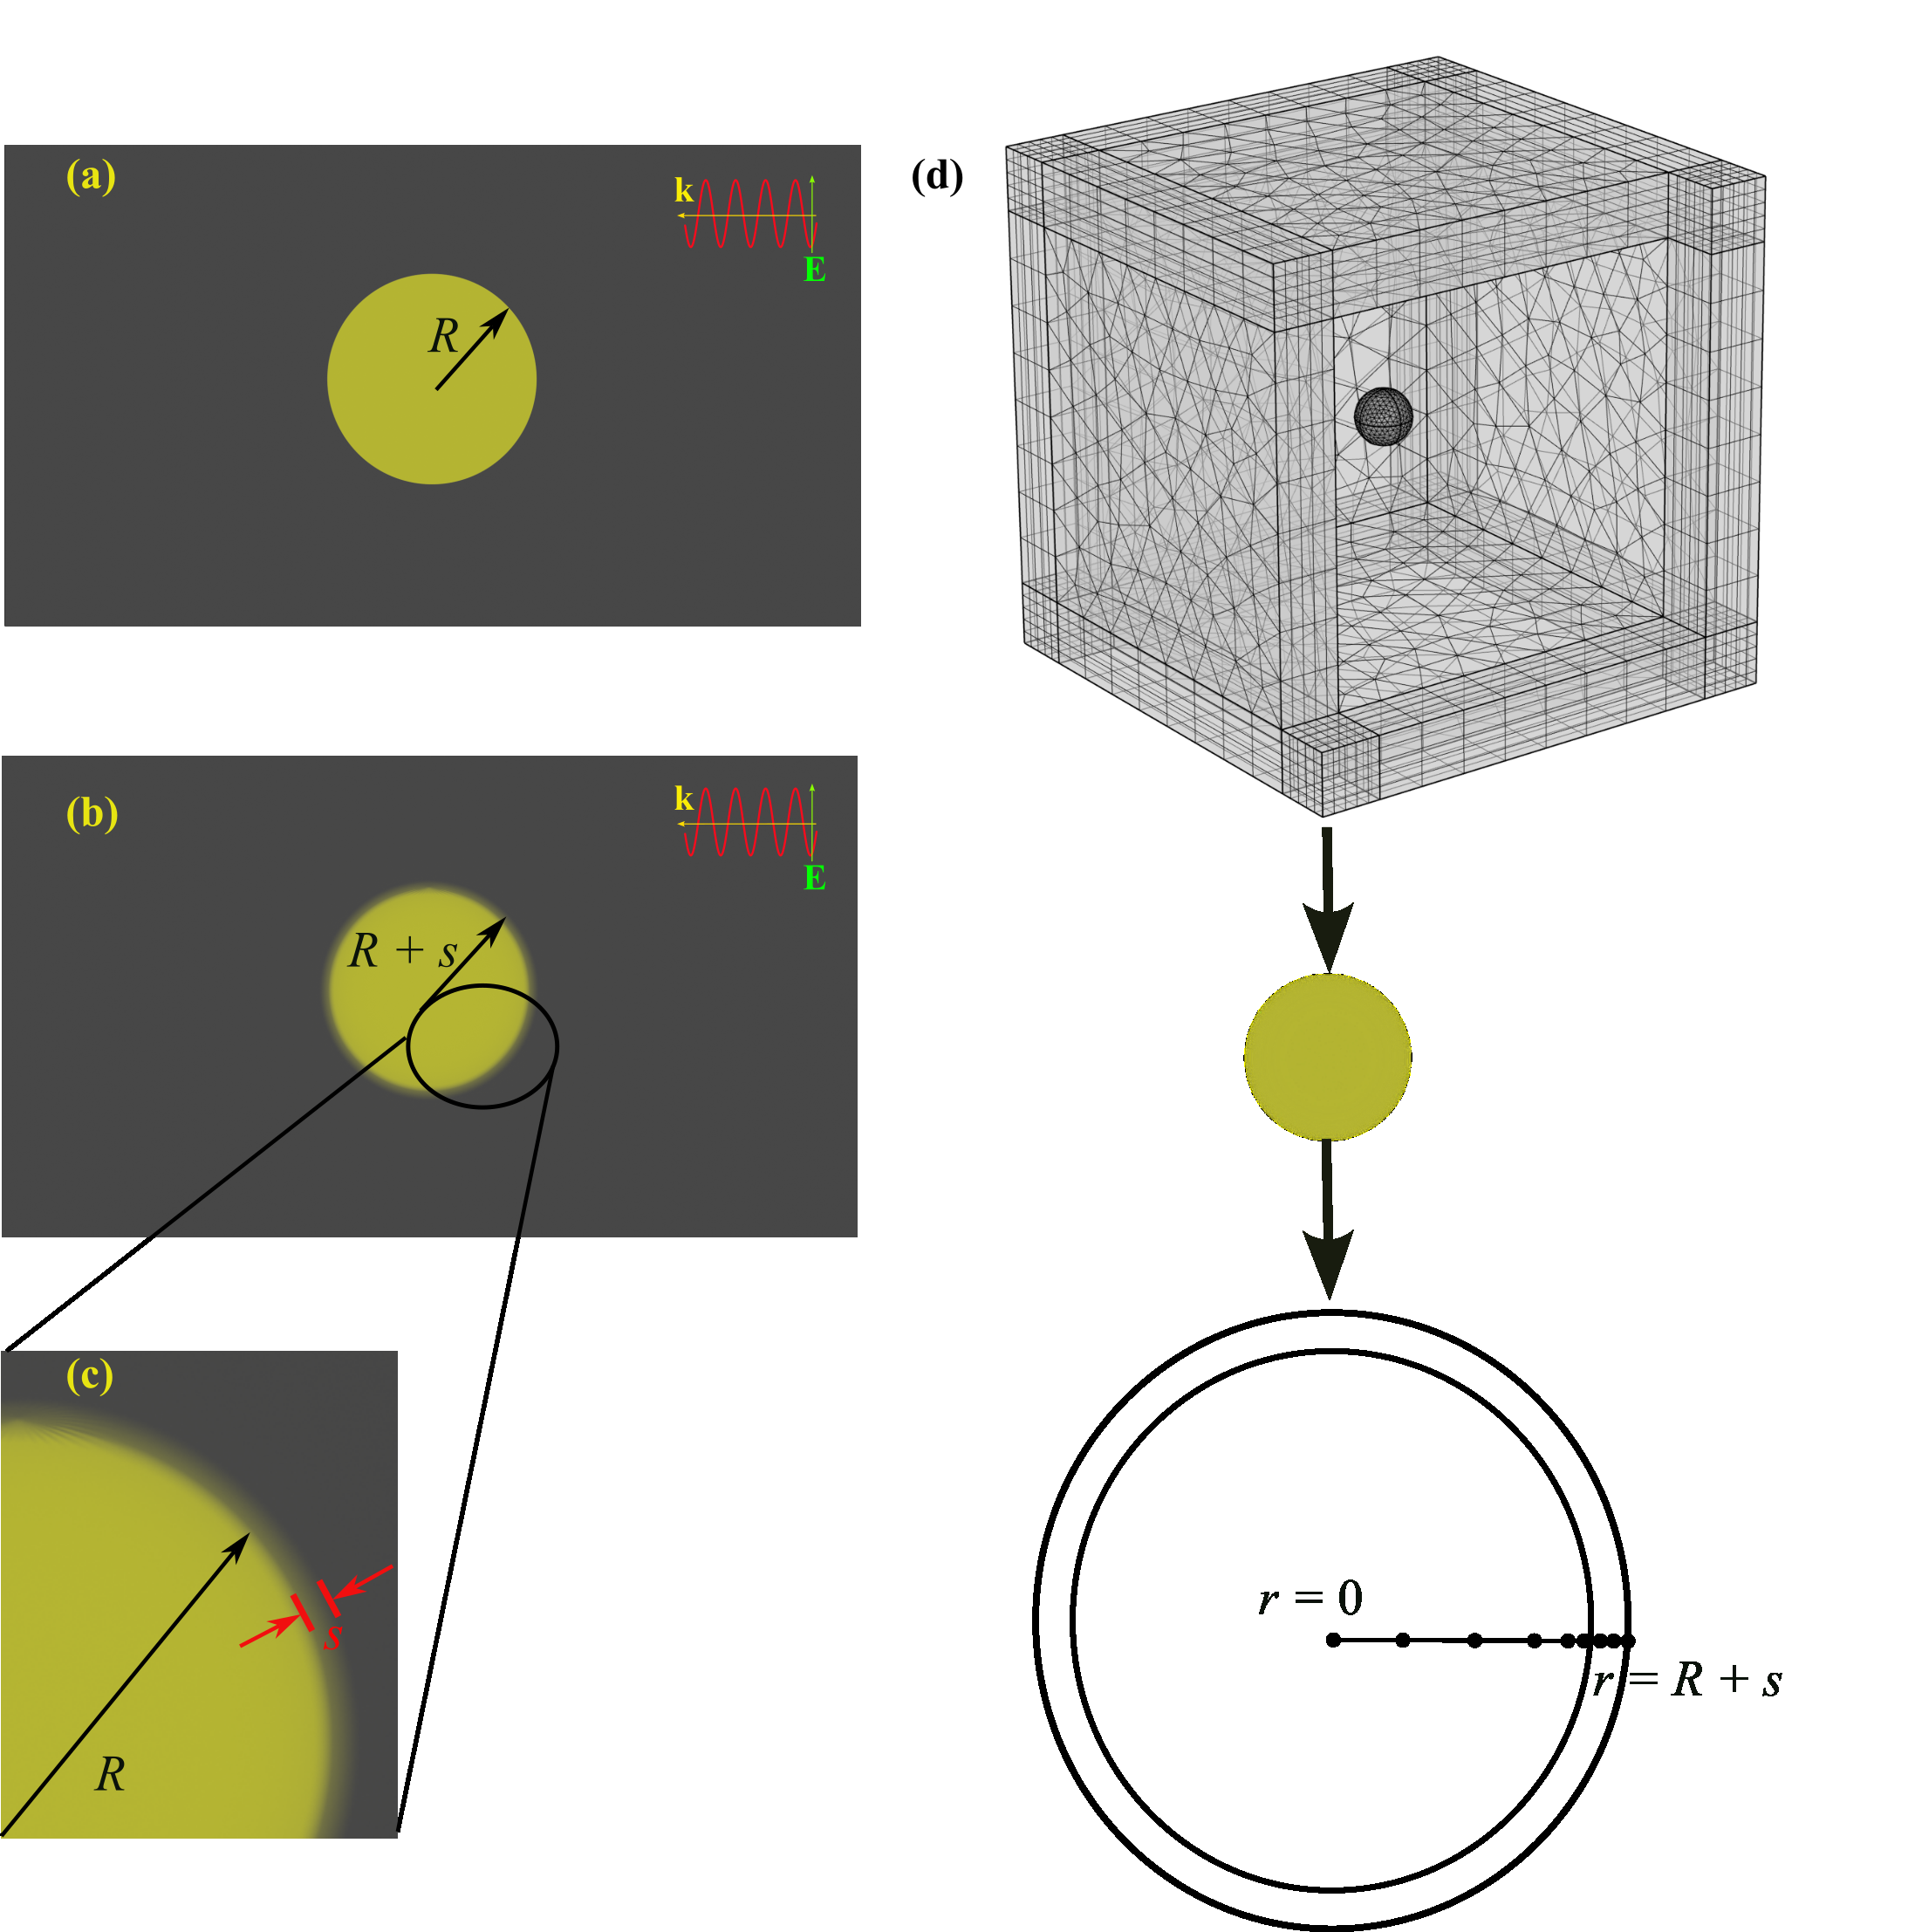
\includegraphics[width=\linewidth,height=0.66\textheight,keepaspectratio]{assets/mystilidis2026_fig1.png}
  \shortcite{C. Mystilidis et al., Nanophotonics 15, e70179 (2026), Fig. 1.}
\end{columns}
\end{frame}

\begin{frame}{The integral solver recovers established LRA and HDM limits}
\footnotesize
\begin{columns}[T,onlytextwidth]
  \column{0.65\textwidth}
  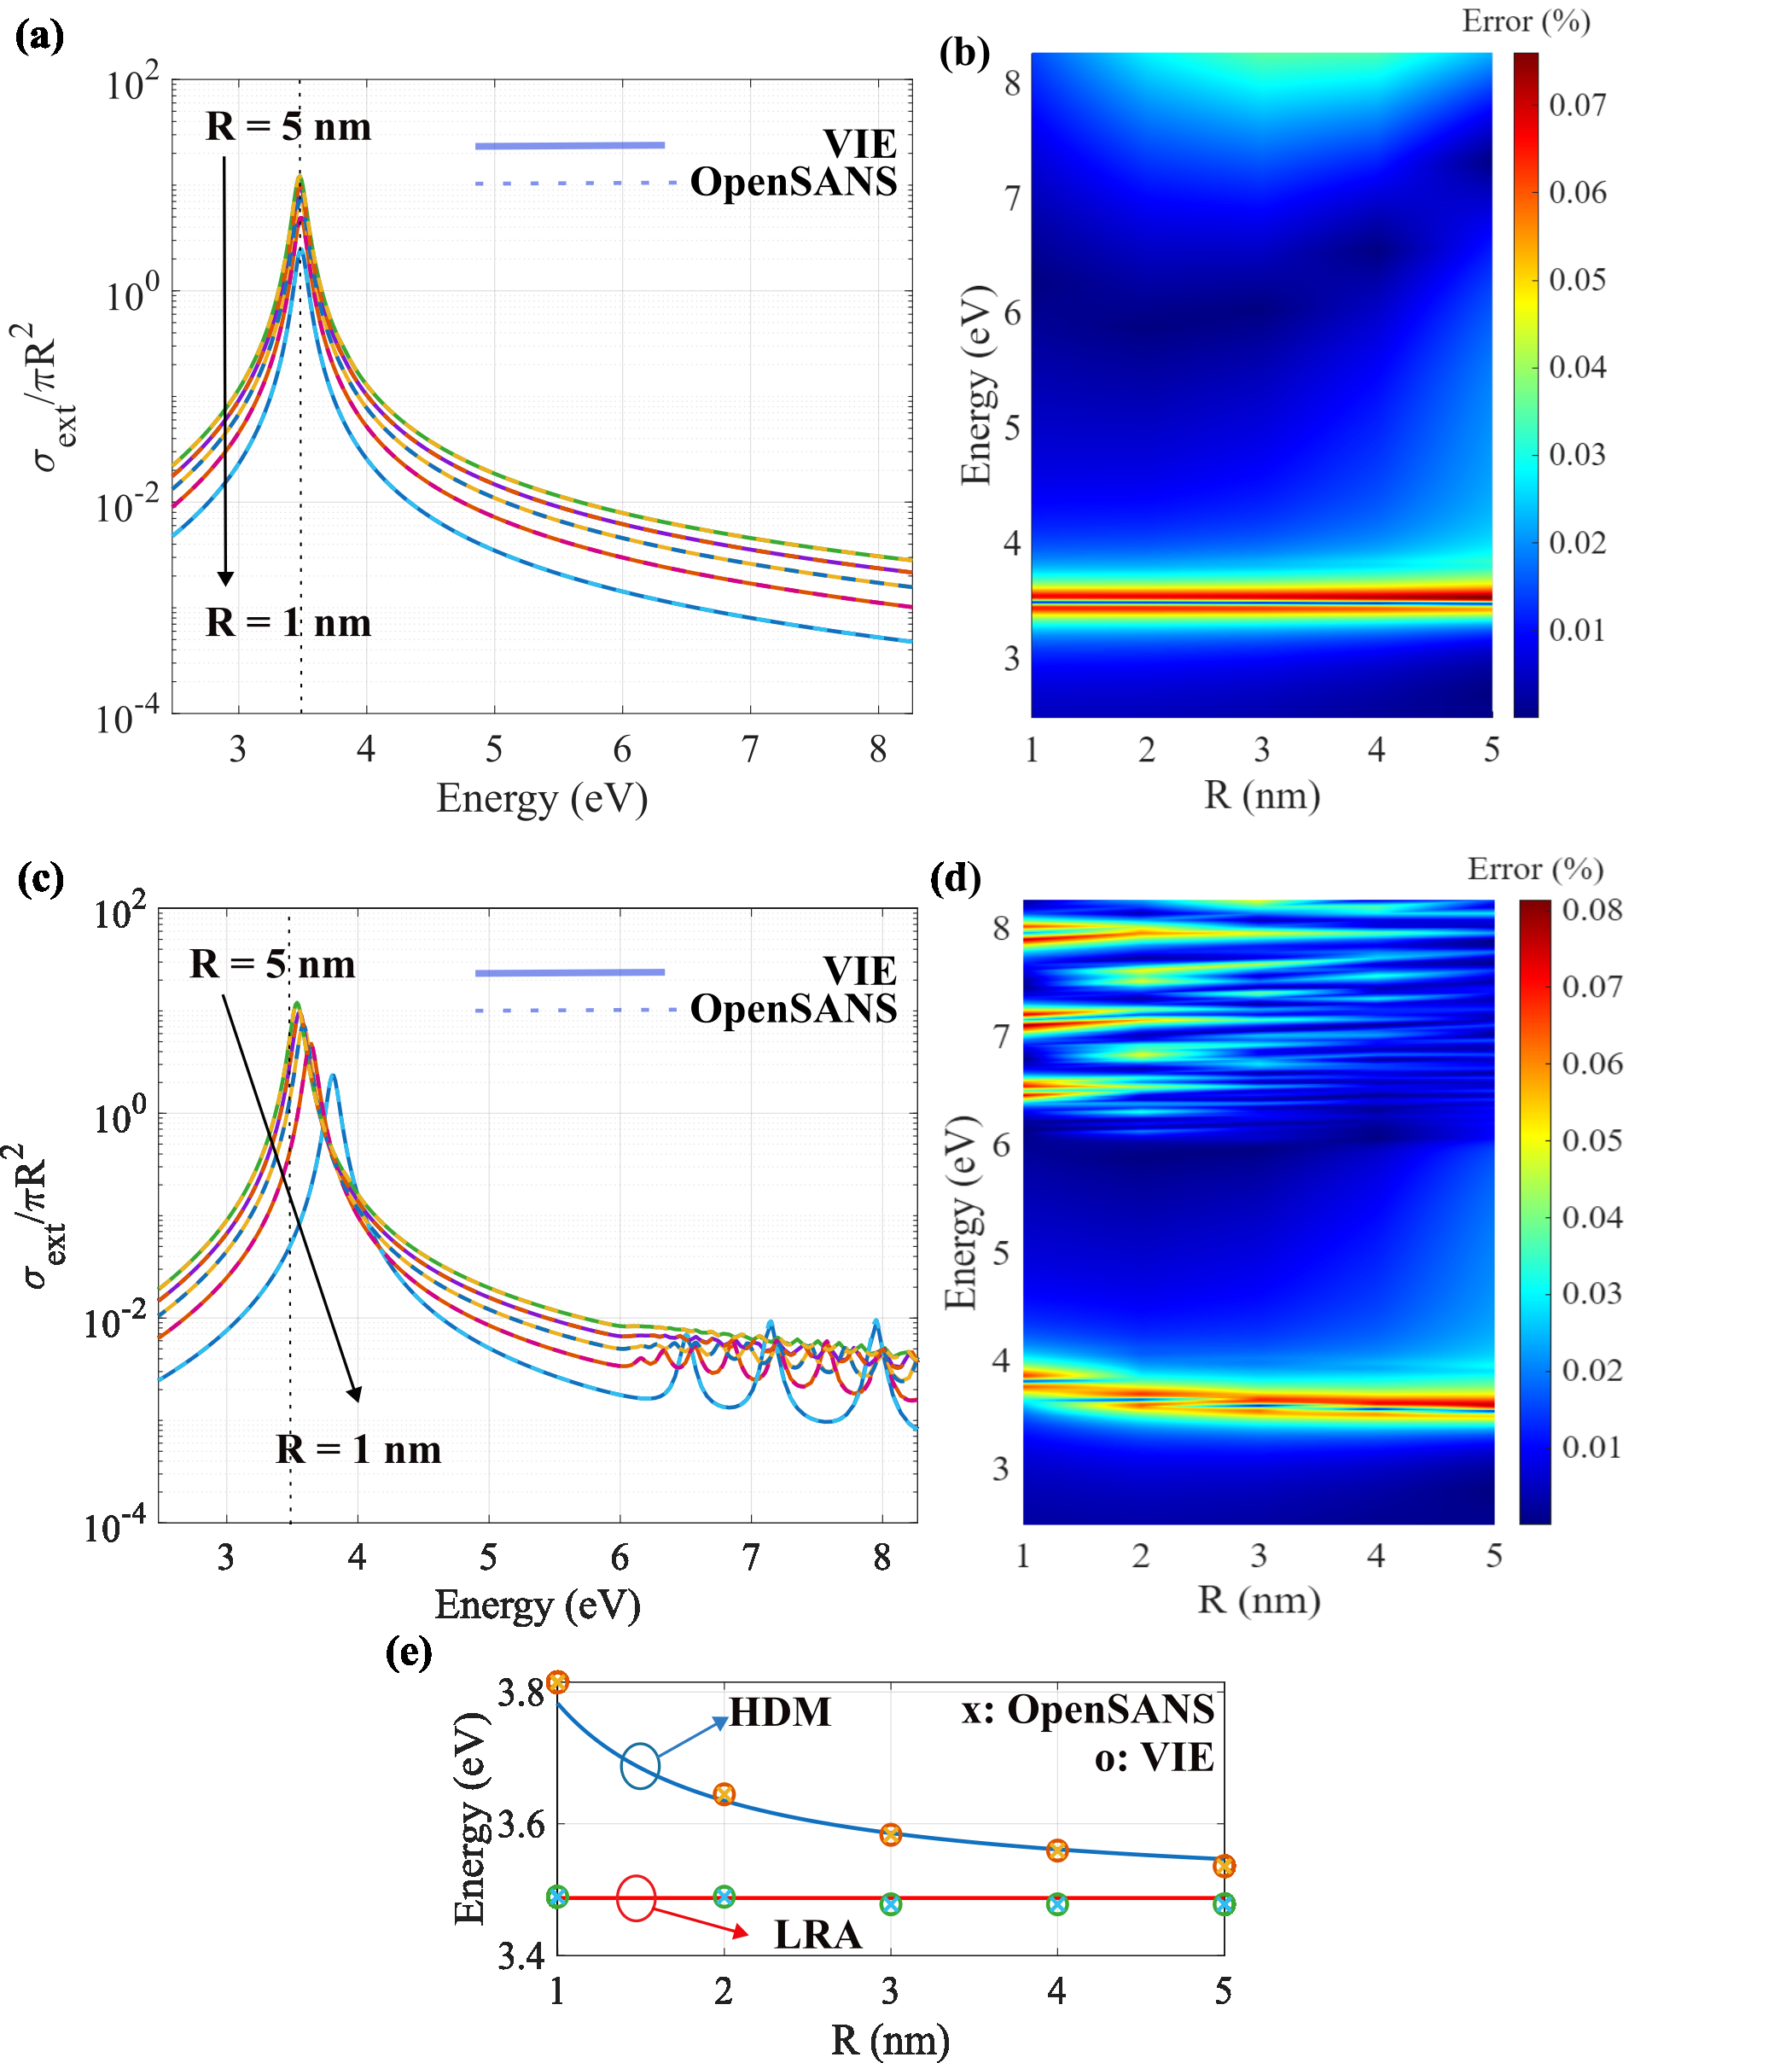
\includegraphics[width=\linewidth,height=0.67\textheight,keepaspectratio]{assets/mystilidis2026_fig2.png}
  \shortcite{C. Mystilidis et al., Nanophotonics 15, e70179 (2026), Fig. 2.}
  \column{0.31\textwidth}
  \begin{block}{Benchmark}
    LRA and hard-wall HDM spectra from the volume-integral formulation track OpenSANS S-matrix results for $R=1$--$5$ nm.
  \end{block}
  \begin{itemize}
    \item Reported relative error is about $0.08\%$ in the benchmark metrics.
    \item The dipolar resonance follows the expected quasistatic radius trend.
  \end{itemize}
  \begin{alertblock}{Scope of the validation}
    The spherical implementation is validated; the SC--HDM material functional is not.
  \end{alertblock}
\end{columns}
\end{frame}

\begin{frame}{Self-consistency redshifts the dipole and reveals a surface mode}
\footnotesize
\begin{columns}[T,onlytextwidth]
  \column{0.66\textwidth}
  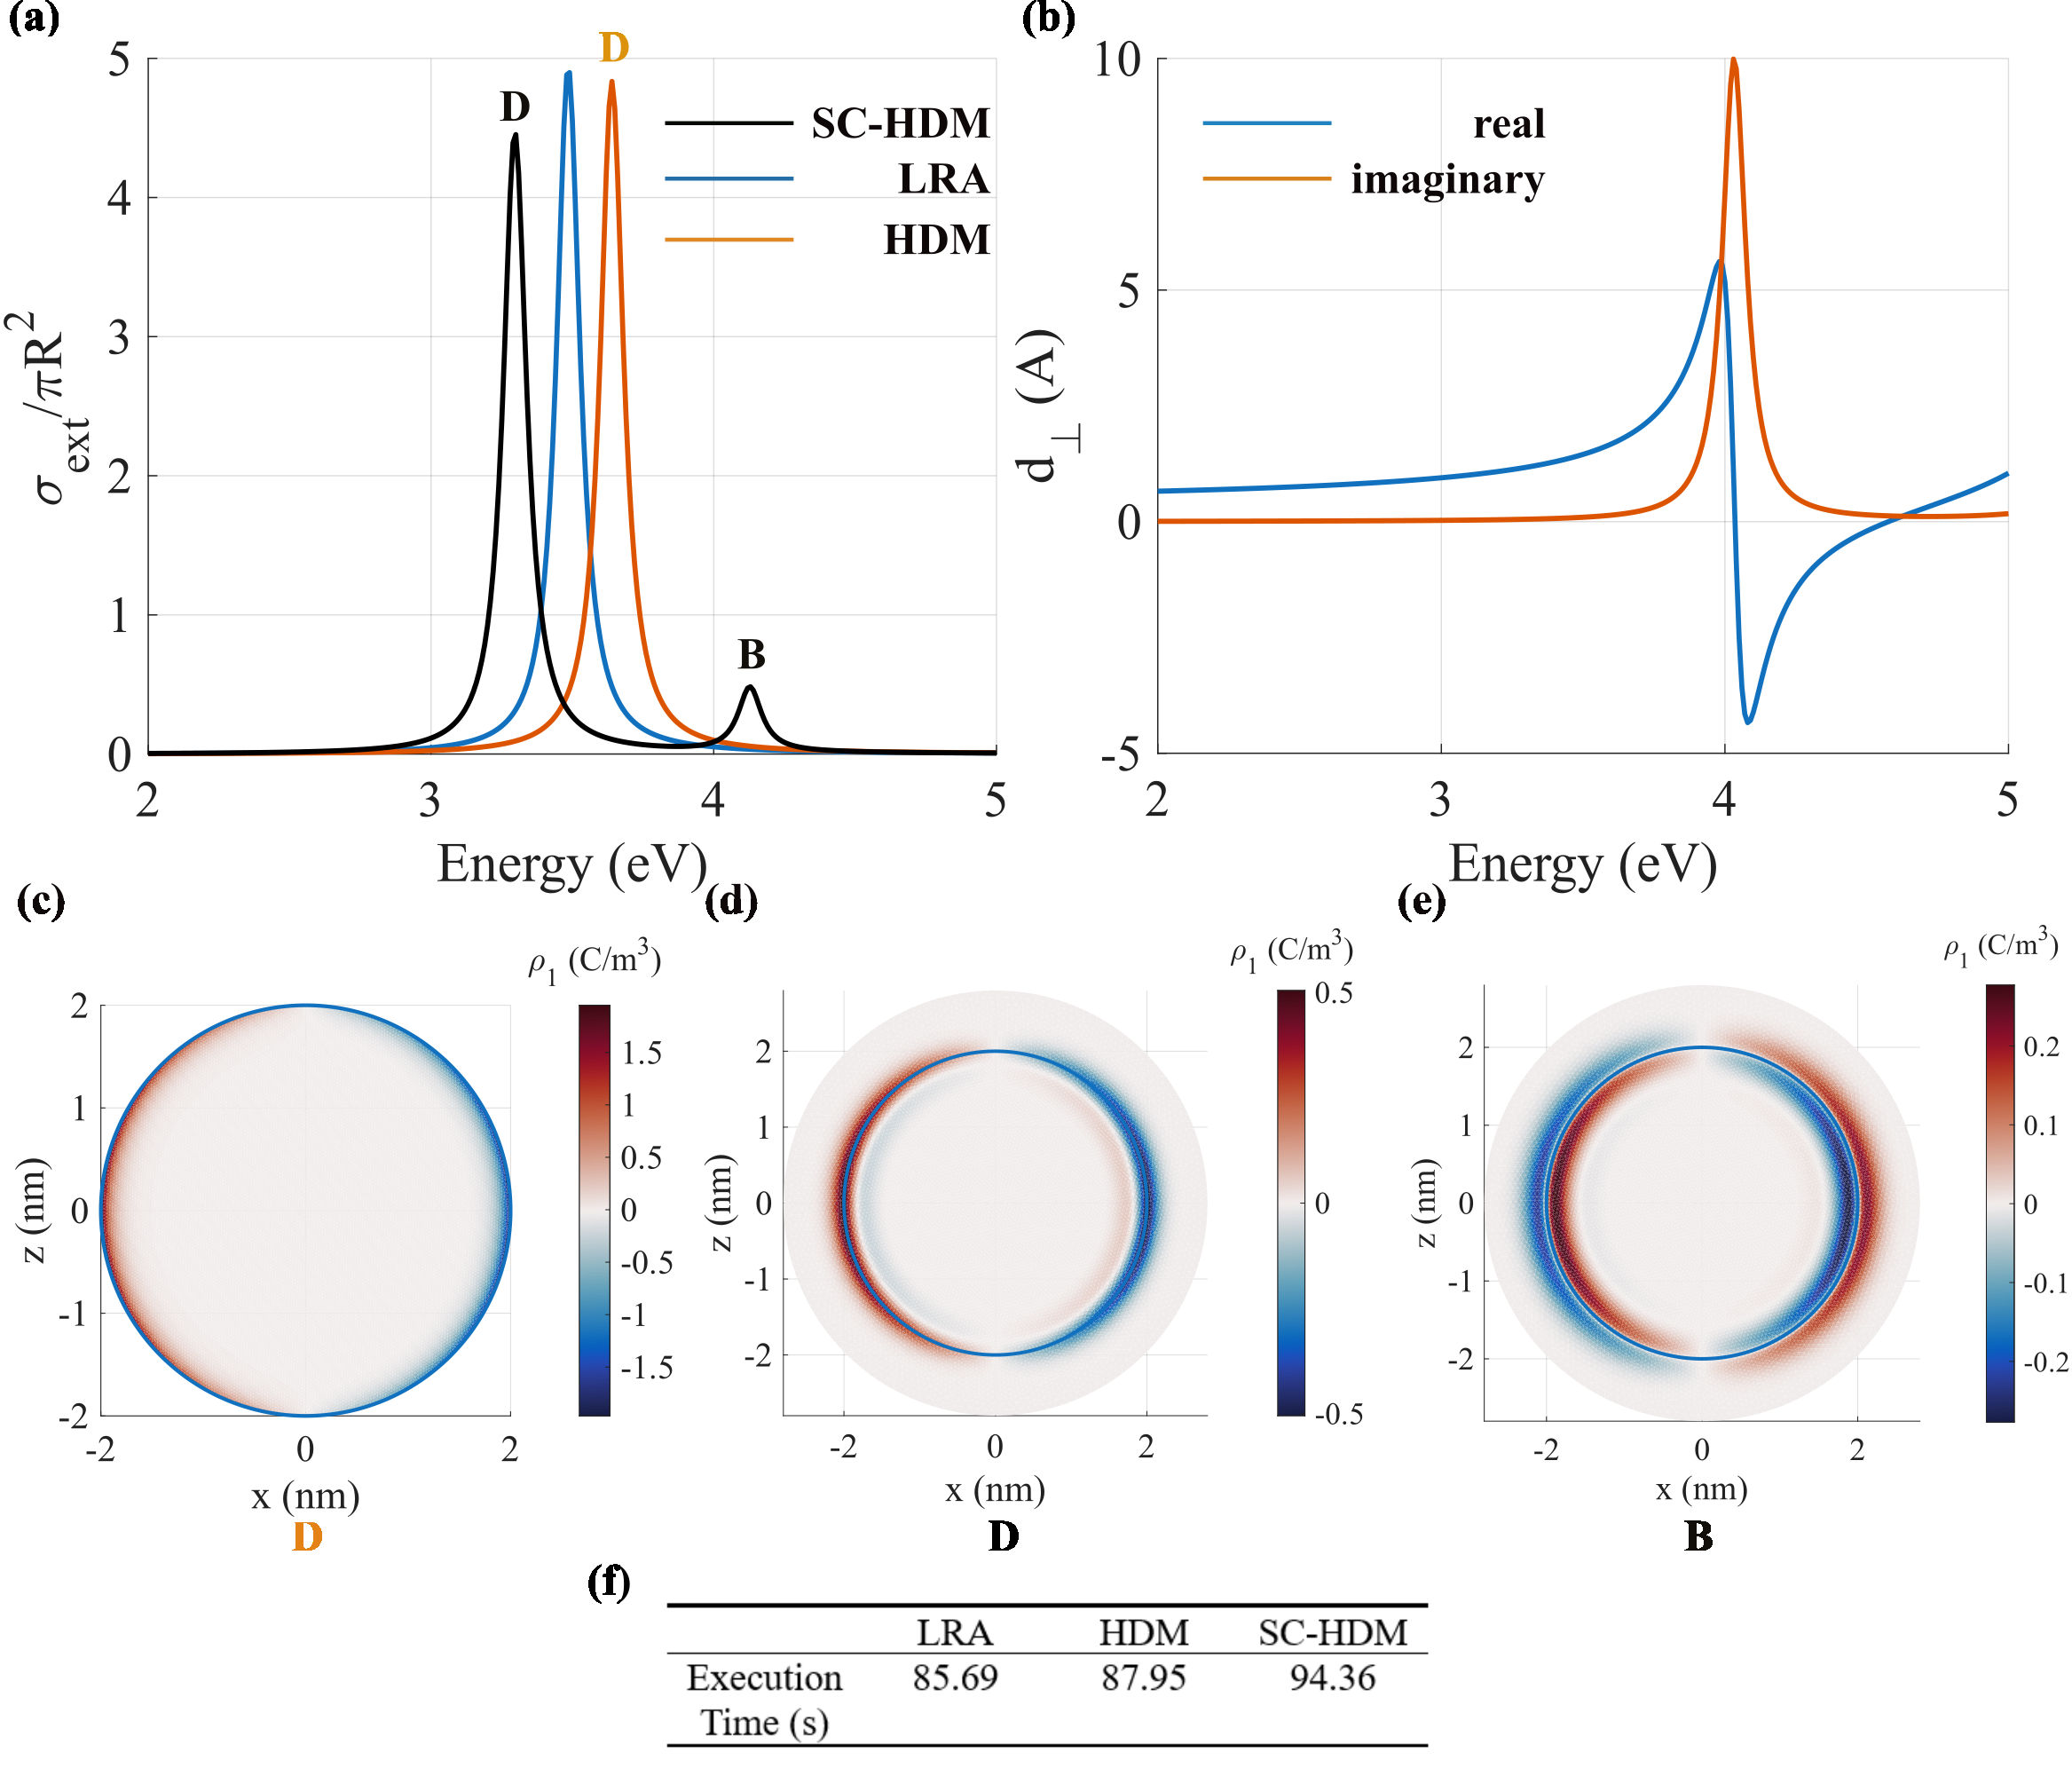
\includegraphics[width=\linewidth,height=0.67\textheight,keepaspectratio]{assets/mystilidis2026_fig3.png}
  \shortcite{C. Mystilidis et al., Nanophotonics 15, e70179 (2026), Fig. 3.}
  \column{0.30\textwidth}
  \begin{block}{For a $2$-nm sodium-like sphere}
    \begin{itemize}
      \item LRA dipole: $\approx3.49$ eV;
      \item hard-wall HDM: $\approx3.64$ eV;
      \item SC--HDM: $\approx3.30$ eV;
      \item Bennett-type feature: near $4.1$ eV.
    \end{itemize}
  \end{block}
  \begin{itemize}
    \item Hard-wall pressure shifts charge inward.
    \item Diffuse $n_0$ moves response outward and reverses the shift.
    \item Charge maps separate dipole and Bennett modes.
  \end{itemize}
\end{columns}
\end{frame}

\begin{frame}{The same calculation can export an effective surface response}
\small
\begin{columns}[T,onlytextwidth]
  \column{0.49\textwidth}
  \begin{block}{From induced charge to a centroid}
    The spherical induced-charge distribution produces a $d_\perp$-like quantity:
    \[
      d_\perp^{\rm sphere}(\omega)
      =\frac{\int (r-R)\rho_{\rm ind}(r,\omega)\,r^2dr}
             {\int \rho_{\rm ind}(r,\omega)\,r^2dr}.
    \]
  \end{block}
  \begin{itemize}
    \item Smooth near the dipole resonance.
    \item Lorentzian structure at the Bennett mode.
    \item A first zero near $4.62$ eV is reported as numerically sensitive.
  \end{itemize}
  \column{0.47\textwidth}
  \centering
  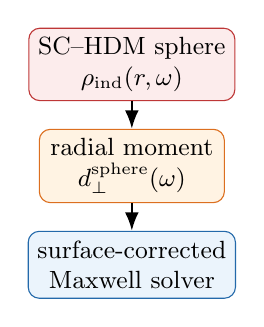
\begin{tikzpicture}[node distance=0.35cm,every node/.style={font=\small,align=center}]
    \node[draw=red,fill=softred,rounded corners,minimum width=2.35cm,minimum height=0.85cm] (a)
      {SC--HDM sphere\\$\rho_{\rm ind}(r,\omega)$};
    \node[draw=orange,fill=softorange,rounded corners,minimum width=2.35cm,minimum height=0.85cm,below=of a] (b)
      {radial moment\\$d_\perp^{\rm sphere}(\omega)$};
    \node[draw=blue,fill=softblue,rounded corners,minimum width=2.35cm,minimum height=0.85cm,below=of b] (c)
      {surface-corrected\\Maxwell solver};
    \draw[-{Latex},thick] (a)--(b);
    \draw[-{Latex},thick] (b)--(c);
  \end{tikzpicture}
  \begin{alertblock}{The transfer is not automatic}
    A finite-sphere centroid is not yet a planar, causal, facet-independent $d(q,\omega)$. Geometry, reference plane, and broadband passivity must be checked.
  \end{alertblock}
\end{columns}
\shortcite{C. Mystilidis et al., Nanophotonics 15, e70179 (2026), Sec. 3.2 and Fig. 3.}
\end{frame}

\begin{frame}{What the spherical bridge still cannot do}
\small
\begin{columns}[T,onlytextwidth]
  \column{0.47\textwidth}
  \begin{block}{Established}
    \begin{itemize}
      \item spherical VIE reproduces LRA and HDM benchmarks;
      \item SC--HDM costs only about 10\% more than LRA in the tested geometry;
      \item diffuse density changes resonance positions and creates a Bennett feature;
      \item the solver can extract a reusable surface-response quantity.
    \end{itemize}
  \end{block}
  \column{0.49\textwidth}
  \begin{alertblock}{Still open}
    \begin{itemize}
      \item arbitrary shapes, edges, substrates, and touching junctions;
      \item noble metals with interband screening and facets;
      \item functional and spill-out-tail calibration;
      \item stable $d(q,\omega)$ transfer to general BEM/FEM geometries;
      \item direct experimental validation of the sodium-like spectra.
    \end{itemize}
  \end{alertblock}
\end{columns}
\vspace{0.35em}
\begin{block}{Interpretation}
  This is a strong solver result and a useful mesoscopic bridge. It is not yet a universal material model.
\end{block}
\shortcite{C. Mystilidis et al., Nanophotonics 15, e70179 (2026).}
\end{frame}

\begin{frame}{A hierarchy of response objects—not a single winner}
\scriptsize
\begin{tabularx}{\linewidth}{@{}p{0.15\linewidth}p{0.19\linewidth}Y Y@{}}
\toprule
\textbf{Model} & \textbf{Response object} & \textbf{Physics retained} & \textbf{Where it stops}\\
\midrule
Local optics & $\varepsilon(\omega)$; $\sigma_{2D}(\omega)$ & geometry, radiation, bulk dispersion and loss & no surface width, $q$ dependence, or transport\\
TDDFT / RPA / GW--BSE / NEGF & $\chi(\mathbf r,\mathbf r';\omega)$ or open-system Green functions & atoms, transitions, excitons, spill-out, tunnelling, correlations & system size and parameter sweeps\\
Feibelman response & $d_\perp(\omega),d_\parallel(\omega)$ & complex interface centroids and surface loss & first-order, interface-local, possibly $q$ dependent\\
HDM / GNOR & density/current fields or $\varepsilon(\mathbf k,\omega)$ & compressibility, longitudinal waves, effective nonlocal loss & hard wall, closure parameters, no chemistry\\
SC--HDM / QHT & $n_0(\mathbf r)$ plus induced $n_1,\mathbf J$ & diffuse equilibrium plus continuum dynamics & functional calibration and multiscale numerics\\
QCM / transport & conductive gap response & tunnelling and charge-transfer plasmons & junction chemistry and transport calibration\\
\bottomrule
\end{tabularx}
\vspace{0.45em}
\begin{alertblock}{For 2D hybrids}
  Keep metal $d$ or QHT response separate from $\sigma_{2D}(q,\omega)$ or excitonic $\chi_{2D}(q,\omega)$; otherwise the fitted ``effective permittivity'' cannot identify which subsystem carries momentum dependence or loss.
\end{alertblock}
\end{frame}

\begin{frame}{From local optics to mesoscopic electrodynamics}
\begin{enumerate}
  \item \key{Local Maxwell theory is the controlled baseline} while every electronic length is small compared with the field-variation scale.
  \item \key{Microscopic calculations reveal the missing physics}—atoms, transitions, facets, spill-out, and tunnelling—but do not scale to device sweeps.
  \item \key{Feibelman parameters compress a thin quantum interface} into complex surface response that can be measured and reused.
  \item \key{Hydrodynamics retains nonlocal density and current dynamics}; self-consistency is needed when the equilibrium surface is diffuse.
  \item \key{The spherical volume-integral formulation makes that bridge practical}, but transfer to realistic materials and arbitrary geometries remains the next test.
\end{enumerate}
\vspace{0.45em}
\begin{block}{The model-selection question}
  Do not ask only, ``Is the system quantum?'' Ask which response object contains the physics that the observable is resolving.
\end{block}
\end{frame}

\end{document}
